\chapter{Methods, Techniques, and Resources}
\label{chap:methods}

%\section{Overview/meta-text}
Here we outline the various existing resources and methods utilised throughout this project. This includes public data repositories, stable and development releases of software packages (mostly for the R programming environment), and implementation of bioinformatics methods or statistical concepts with Shell or R scripts developed for this purpose. Methods and packages developed specifically for this project will be covered in more detail along with preliminary data to demonstrate and support their use in the following chapter. 

\section{Bioinformatics Resources to Enable Genomics Research}
\subsection{Public Data and Software Packages}
Various bioinformatics resources, such as databases and methods, have become an integral part of genetics and genomics research. Reference genomes, genotyped variants, gene expression, and epigenetics profiles are among the most commonly used resources. Gene expression in particular is widely available from many microarray and RNA-Seq studies, including Gene Expression Omnibus (GEO), caArray, and arrayExpress. Such profiles serve as an excellent resource to examine the changes of gene expression occurring in cancers and their variation. These microarray initiatives have set a precedent for data sharing, data mining, and the wider benefits of publicly available data for enabling the scientific community further utilise the data compared to a single research group or consortium. The practice of integrating findings from publicly available genomics data with the research questions and experimental results of individual research groups has carried over into RNA-Seq datasets including the large-scale cancer genomics projects (such as TCGA). This thesis is one such example of an investigation enabled by this wider movement and tools developed in various disciplines to generate, disseminate, and process genomic-scale data.
 
Along with databases, it is also becoming common practice for Bioinformatics researcher to release their code open-source or provide a software package to enable replication of the findings or further applications of the methods. This is part of a wider movement in software and data analysis with many tools to facilitate such work being released for use in Linux or the R programming environment. In addition to the R packages hosted on CRAN, the Bioconductor repositories also contain many packages specifically for applications in Bioinformatics, and the GitHub site hosts many packages in various stages of development and early release. Packages from these various sources have been used throughout this project and cited where-ever possible. Several R packages have been developed during this thesis project and either publicly released on GitHub or prepared to accompany a publication.

\subsubsection{Cancer Genome Atlas Data}
Moelcular profile data from normal and tumour samples was downloaded from publicly available sources, using the TCGA \cite{TCGA2012} and the International Cancer Genome Consortium (ICGC) web portals \cite{ICGC2011}. These include gene expression (RNA-Seq), somatic mutations, and anonymous clincal data. The latest versions downloaded were on Aug 6th 2015 (Release 19) and May 2nd 2016 (Release 20) for breast and stomach cancer respectively via the ICGC data portal.
%%The Cancer Genome Altas project supports a wide range of cancers including gene expression for breast invasive adenocarcinoma with 600 samples (63 normal, 534 primary tumour, and 3 metastases) available the AligentG4502 244K cDNA microarray mapping 17811 genes \cite{TCGA2012}. TCGA provides microarray expression data processed with loess normalisation and integrated to give an expression call for each gene. %% Array data removed

There remains debate regarding the optimal methods to perform an alignment. However, the statistical and biological aspects of Bioinformatics are the focus of this thesis, comparing alignment methods is outside the scope of this investigations. The TCGA project used the widely adopted ``Bowtie'' tools for alignment, with ``mapslice'' to detect splice sites, and the Reads Per Kilobase per Million mapped reads (RPKM) approach to qualify reads per transcript as a measure of gene expression. These are widely acceptable tools for processing RNA-Seq data and this is the raw quatitative expression data publicly available from TCGA.

Raw count and RSEM normalised TCGA expression data from Illumina RNA-Seq protocols were available from 1,177 samples (113 normal, 1,057 primary tumour, and 7 metastases) for 20,501 genes. TCGA somatic mutation data for 981 samples (976 primary tumours and 5 metastases) across 25,836 genes were available including 969 samples (964 primary tumours and 5 metastases) with corresponding RNA-Seq expression data and 19,166 genes mapped from Ensembl identifiers to gene symbols, of which 16,156 had corresponding gene expression information. Unless otherwise stated, the raw counts were used for further processing rather than the RSEM normalised data provided by TCGA tier 3.

\subsubsection{Reactome and Annotation Data} \label{methods:gene_set}

Unless otherwise specified, pathway analysis was performed for Human pathway annotation from the Reactome database (version 52) with pathway gene sets derived from the \texttt{reactome.db} R package. Entrez identifiers were mapped to gene symbols or aliases to match to TCGA expression and mutation data using the \texttt{org.Hs.eg.db} R package. Further pathway analysis used breast cancer gene signatures from Gatza and colleagues (Gatza \textit{et al}., 2011; Gatza \textit{et al}., 2014). These gene symbols were matched to the relevant dataset and used to construct a matrix of category membership using the \texttt{safe} R package \cite{safe}.

\section{Data Handling}

\subsection{Normalisation (voom)}

Apart from the PAM50 subtyping procedure \cite{Parker2009} which required RSEM normalised data as (J.S. Parker personal communication), the analysis of the RNA-Seq data presented here was based on raw read count data. Raw read counts were log-scaled, samples were trimmed as described above based on a correlation matrix (Euclidean distance), and the final dataset was TMM normalised \cite{Robinson2010} and then processed using the \texttt{voom} function \cite{Law2014} in the \texttt{limma} R package \cite{limma}.

\begin{figure*}[!ht]
%  \resizebox{\textwidth}{!}{
         \begin{center}
%
        \subfigure[Raw counts (log-scale)]{%
            \label{fig:first}
            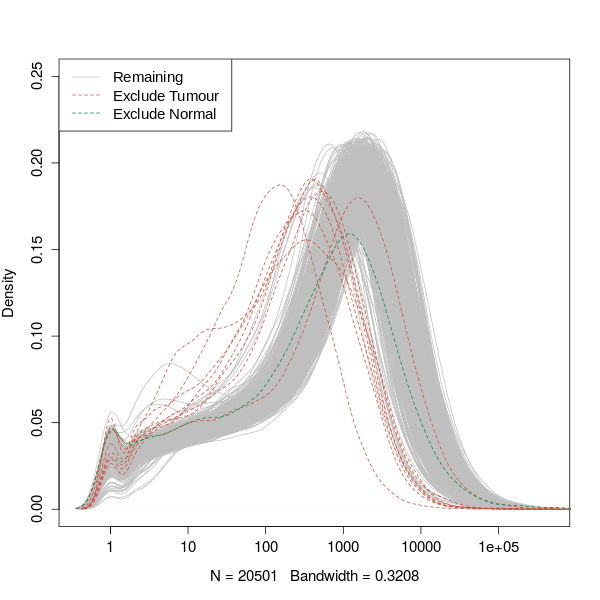
\includegraphics[width=0.4\textwidth]{fig2a.png}
        }%
        \subfigure[Voom normalised]{%
           \label{fig:second}
           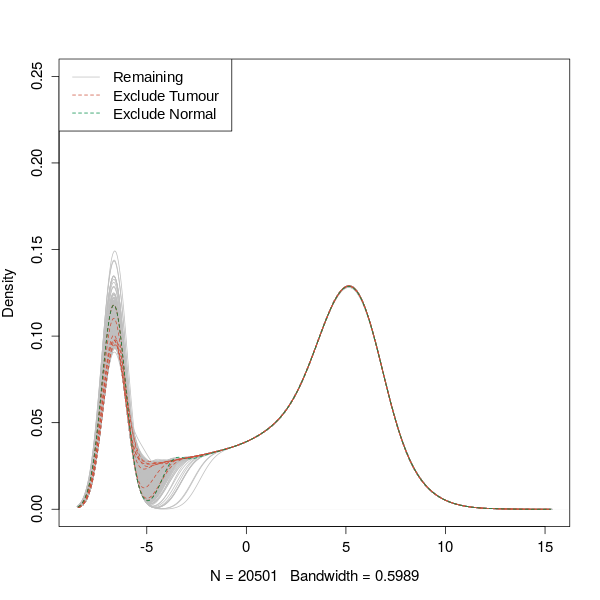
\includegraphics[width=0.4\textwidth]{fig2b.png}
        }%
%
    \end{center}
   \caption[Read count density]{\textbf{\csentence{Read count density.}} Sample density plots of raw counts on log-scale and voom normalised showing samples removed due to quality concerns.}
%}
\label{fig:density}
\end{figure*}

\begin{figure*}[!ht]
%  \resizebox{\textwidth}{!}{
         \begin{center}
%
        \subfigure[Mean raw counts (log-scale)]{%
            \label{fig:first_mean}
            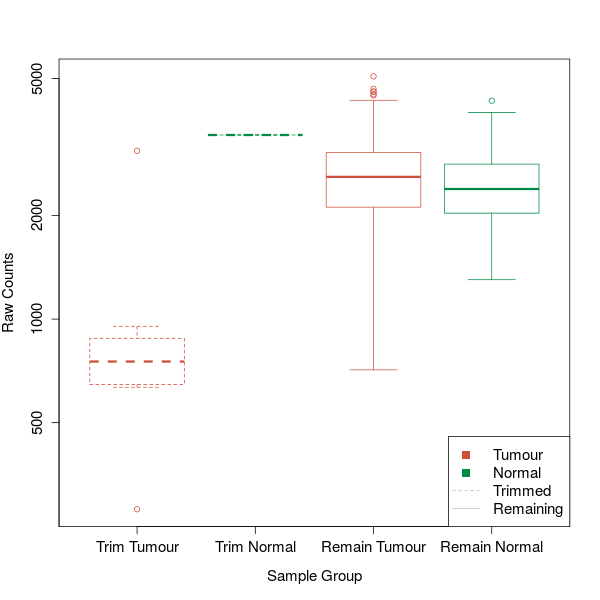
\includegraphics[width=0.4\textwidth]{fig3a.png}
        }%
        \subfigure[Mean voom normalised]{%
           \label{fig:second_mean}
           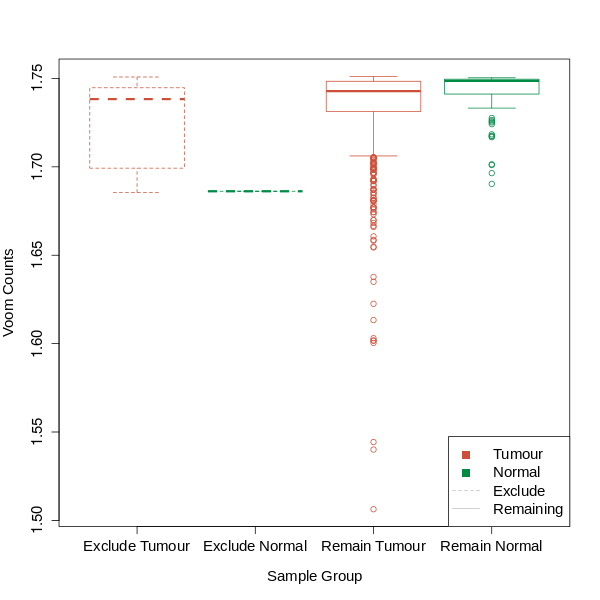
\includegraphics[width=0.4\textwidth]{fig3b.png}
        }%
%
    \end{center}
  \caption[Read count sample mean]{\textbf{\csentence{Read count sample mean.}} Sample boxplots of raw counts on log-scale and voom normalised showing samples removed due to quality concerns with low sample mean read count.}
%}
\label{fig:boxplot}
\end{figure*}


\subsection{Sample triage}

The TCGA RNA-Seq data were assessed for batch effects using a correlation matrix of the log-transformed raw counts for which a heatmap (Euclidean distance, complete linkage) is shown in Figure \ref{fig:corr_map}. While no major batch effects were detectable between the samples, 9 samples were excluded due to poor correlation with the remaining samples as detailed in Table \ref{tab:qc}. These samples show unusual density plots compared to the rest of the dataset and low mean read count in Figures \ref{fig:density} and \ref{fig:boxplot}. A heatmap showing key clinical properties of these excluded samples and their correlation with other rest of the samples is shown in Figure \ref{fig:corr_map_part} and a full correlation heatmap (Figure \ref{fig:corr_map}) shows these samples as relatively poorly correlated outliers in the bottom rows and left columns.
%In both of these cases, a shared tissue source site or patient donor indicates that variations in sample preparation are likely behind the outlying expression profiles. The Christiana Healthcare patients were sequenced in triplicate when replicate samples were rare in this dataset suggesting there were suspected errors in these samples during data generation which have lower mean read count than most of the dataset. %tangent
%Clinical characteristics over-represented in removed samples were ER+, ductal, state 2, luminal A or basal type tumours but these are the most common in the dataset. %relevance
After removal of these samples, the TCGA dataset used for analysis consisted of the remaining 1168 samples (from 1040 patients): 1049 tumour samples, 112 normal tissue for matched samples, and 7 metastases.

\begin{table*}[!ht]
\caption{Excluded samples batch and clinical characteristics.}
\label{tab:qc}
\resizebox{\textwidth}{!}{
      \begin{tabular}{|c|c|c|c|c|c|c|c|c|ccc|}
        \hline
        Tissue Source		& Type   & Batch & Plate & Patient & Samples & p53      & Subtype   & Treatment (History) 			& \multicolumn{3}{ c| }{Clinical (Stage)} \\ \hline
        A7 Christiana		& Tumour & 47	 & A227  & A0DB  &  1 of 3   & NA       & Luminal A & Mastectomy (no)				& ER+  &  Ductal   	& (2)        \\
        A7 Christiana		& Tumour & 96	 & A220  & A13D  &  1 of 3   & Wildtype & Luminal A & Mastectomy (no)				& ER+  &  Ductal   	& (2)        \\
        A7 Christiana		& Tumour & 96	 & A227  & A13E  &  1 of 3   & NA       & Basal     & Lumpectomy (no) 				& ER-  &  Ductal   	& (2)        \\
        A7 Christiana		& Tumour & 142	 & A277  & A26E  &  1 of 3   & NA       & Basal     & Lumpectomy (no) 				& ER+  &  Ductal   	& (2)        \\
        A7 Christiana		& Tumour & 47	 & A277  & A0DC  &  1 of 2   & NA       & Luminal A & Mastectomy (yes)				& ER+  &  Lobular   	& (3)        \\
        A7 Christiana		& Tumour & 142	 & A220  & A26I  &  1 of 2   & Mutant   & Basal     & Lumpectomy (yes) 				& ER-  &  Ductal   	& (2)        \\
        AC Intl Genomics	& Tumour & 177	 & A18M  & A2QH  &  2 of 2   & Mutant   & Basal     & Radical Mastectomy (no) 			& ER-  &  Metaplastic   & (2)        \\
        AC Intl Genomics	& Tumour & 177	 & A220  & A2QH  &  2 of 2   & Mutant   & Basal     & Radical Mastectomy (no) 			& ER-  &  Metaplastic   & (2)        \\
        GI ABS IUPUI		& Normal & 177	 & A16F  & A2C8  &  1 of 1   & NA       & Luminal A & Radical Mastectomy and Neoadjuvant (no) 	& ER+  &  Ductal   	& (2)        \\ \hline
      \end{tabular}
}
\end{table*}

\begin{figure*}[!ht]
  \resizebox{0.95 \textwidth}{!}{
    \includegraphics{Raw(log)_Corr_eudist_Cut_part_Pub.png}
   }
   \caption[Correlation profiles of removed samples]{\csentence{Correlation profiles of removed samples.} Correlation matrix heatmap (Euclidean distance) of all samples in TCGA breast cancer dataset on the left (clustered with respect to all samples) against those removed annotated for sample codes: tissue source site (TSS), sample type with reds for tumour and greens for normal, patient showing both A2QH samples in pink, with various colours for analyte and plate (corresponding to batch in Table \ref{tab:qc}). Trimmed samples cluster at the bottom of the heatmap and the colour bars of the left therefore show which sample properties are shared with other samples in the dataset.)}
\label{fig:corr_map_part}
\end{figure*}

\begin{figure*}[!ht]
  \resizebox{\textwidth}{!}{
    \includegraphics{Raw(log)_Corr_eudist_Ann_Pub.png}
   }
   \caption[Correlation analysis and sample removal]{\csentence{Correlation analysis and sample removal.} Correlation matrix heatmap (Euclidean distance) of all samples in TCGA breast cancer dataset against each other annotated for sample clinical data: sample type, tissue type, tumour stage, Estrogen receptor (IHC) and intrinsic subtype (from the PAM50 method). CDH1 somatic mutation, gene expression, and status for SLIPT prediction are also annotated. Discrete variables are coloured as displayed in the legend and continuous variables on a blue-red scale as shown in the colour key. Trimmed samples cluster at the bottom of the heatmap and the colour bars of the left show which were removed for quality concerns.)}
\label{fig:corr_map}
\end{figure*}

\subsection{Pathway Metagenes and the Singular Value Decomposition} \label{methods:metagene}
A ``metagene'' offers a consistent signal of pathway (expression) activation or inactivation by dimension reduction of a matrix, rather than negatively correlated genes averaging out the signal \cite{Huang2003}. Construcing these pathway metagenes used gene sets for Reactome and Gatza signatures (Gatza \textit{et al}., 2011; Gatza \textit{et al}., 2014) as specified above (see Section \ref{methods:gene_set}). The singular-value decomposition was performed ($X = U^{T} D V$ where $X$ is the data matrix of the gene set with genes $\times$ samples) and the leading eigenvector ($V[,1]$) corresponding to the largest singular value was used as a metagene for the pathway gene set. To ensure consistent directionality of metagene signals, the median of the gene set in each sample was calculated and correlated against the metagene with the (arbitrary) metagene direction is reversed to conform with the majority of the gene set. To ensure that genes and pathways were weighted equally, this was performed on a z-transformed dataset of gene expression and samples were ranked for each metagene so that each metagene was on a comparable $[0,1]$ scale. 

\subsubsection{Candidate Triage and Integration with Experimental Data} \label{methods:venn_analysis}
Candidate triage in combination with the experimental data was intended to integrate findings of the SLIPT analysis with an ongoing experiment project \cite{Chen2014, Telford2015}. The first procedure to compare the SLIPT gene candidates for \textit{CDH1} with an siRNA experimental screen \cite{Telford2015} was a direct comparision of the overlapping candidates, presented in a Venn diagram and tested with the $\chi^2$ test. Since these candidates were not very comparable at the gene level (even when excluding genes not contained in both datasets), further gene set over-representation analysis was performed for pathways specific to each detection approach and the intersection of the two. The pathway composition of the intersection was further verified by a permutation resampling analysis (as described in section \label{methods:permutation}), the same number of genes detected by SLIPT were sampled randomly from the universe of genes tested by both approaches. These samplings were performed over 1 million iterations and the pathway over-representation was compared for each of the 1,652 reactome pathways. Adjusting for multiple comparisions was not needed here in a permutation analysis as the test $\chi^2$ statistics were directly used with the same degrees of freedom between expected and observed. These over-representation scores ($\chi^2$) were compared the observed over-representation in the intersection of the SLIPT candidates, with the proportion of resamplings with higher $\chi^2$ values used for empirical p-values of pathway composition. These empirical p-values were adjusted for multiple comparisions (FDR) and pathways for which no resamplings were observed as high as the observed were assumed to be zero for the purposes of FDR and reported as less than the adjusted value of one in a million resamplings. Intersection size was not assumed to be constant across resamplings so similarly with the proportion of resamplings with higher or lower intersection size were used to evaluate significance of enrichment or depletion respectively (of siRNA candidate among SLIPT candidate genes).  

\section{Techniques}
Various statisical, computational, and bioinformatics techniques were performed throughout this thesis. This section presents these techniques and where relevant acknowledges the R package implementation which provided it and gives the parameters used in data presented in the thesis unless otherwise specified.

\subsection{Statistical Procedures and Tests}

As described in sections \ref{methods:heatmap} and \ref{methods:metagene}, the z-transform has been used to generate z-scores in various analyses in this thesis. Here the each row of dataset ($x$) is transformed into a scores ($z$) using the mean ($\mu$) and standard deviation ($\sigma$) of the data such that: $$ z = \frac{x - \mu(x)}{\sigma(x)} $$. This generates data where each row (gene) has a mean of 0 and standard deviation of 1. Where plotted as heatmap, any data more than 3 standard deviations from the mean is plotted as 3.

Differential expression analysis was performed with empirical Bayes, using the \texttt{limma} R package \cite{limma}. Where specfied, the Fisher's exact test, $\chi^2$ test, and correlation are used to measure associations between variables (as implemented in the \texttt{stats} R package \cite{R_core}). Unless otherwise specified, Pearson's correlation is used for correlation analyses ($r$) and coefficient of determination ($R^2$). Where these comparisons are discussed in more detail, Fisher's exact test and $\chi^2$ tests will be supported by a table or Venn diagram, rendered with the \texttt{limma} R package \cite{limma}. Correlation analyses may be supported by a scatter plot and a line of best fit dervied by least squares linear regression. 

The \texttt{t.test} function \cite{R_core} has also been used to implement the t-test to compare pairs of data. Where these have been typically supported by visualisation of a boxplot rendered in R. Where relevant an analysis of variance (ANOVA) has been performed to report significance of multivariate predictors of outcomes or least squares linear regression performed for the adjusted coefficient of determination ($R^2$) and f-statistic p-value to evaluate the fit of the predictor variables.

Multiple comparisons are adjusted by Benjamini-Hochberg procedure to control the false discovery rate (FDR) unless otherwise specified \cite{fdr1995}. This procedure adjusts p-values to an estimate of the proportion of false-postives among tests with this p-value or lower. The more stringent Holm-Bonferroni (Holm) procedure \cite{Holm1979} was also applied in some cases to adjust for multiple comparisons by the family-wise error rate which adjusts p-values to the probability that any one of the tests with this p-value or lower is negative.

\subsection{Gene Set Over-representation Analysis}
Gene set enrichment over-representation tests whether there is an enrichment of a gene set (such as a biological pathway) among a group of input genes. Such input genes may be predicted synthetic lethal candidates or a subset as defined by clustering (in section \ref{methods:clustering}) or comparison with experimental candidates (see section \ref{methods:venn_analysis}). Initially, these were performed using the GeneSetDB web tool \cite{genesetdb} hosted by the University of Auckland on the Reactome pathways \cite{reactome}. Since the GeneSetDB tool used an older version of Reactome (version 40), it was difficult to directly compare with the results of other analysis (see sections \ref{methods:venn_analysis} and \ref{methods:permutation}) performed on version 52 (as described in  section \label{methods:gene_set}). Thus an implementation of the hypergeometric test in R \cite{R_core} was used to test for over-representation against Reactome (version 52) pathways. Pathways containing less than 10 genes or more than 500 (as performed in GeneSetDB \cite{genesetdb}) were excluded before adjusting for multiple comparisons.

\subsection{Clustering} \label{methods:clustering}
Clustering analysis when performed uses unsupervised hierarchical clustering with complete linkage (distance calculated from the furthest possible pairing). When data has been generated relates to correlations, such as correlation matrices or Sigma (multivariate normal) parameters, the distance measure used was Euclidean distance. For empirical or simulated gne and pathway expression data correlation distance is used, calculated by $distance = 1 - cor(t(x))$ where \texttt{cor} is Pearson's correlation and \texttt{t(x)} is the transpose of the expression matrix. 

\subsection{Heatmap} \label{methods:heatmap}
Standardised z-scores of the data were used to plot heatmaps on an appropriate scale. Raw (log-scale) read counts or voom normalised counts per gene (as specified) were plotted  as normalised z-scores on a $[-3,+3]$ blue-red scale. Similarly, correlations were plotted on a $[-1,1]$ blue-red scale. These heatmaps were performed using the linkage and distance specified for the clustering performed in Section \ref{methods:clustering}. The \texttt{gplots} R package \cite{gplots} was used to generate many of the heatmaps throughout this thesis, along with a customised heatmap function (released as \texttt{heatmap.2x}). Where clearly specfied, data has been split with clustering performed separately on each with these plotted alongside each other.

\subsection{Modeling and Simulations}
Statisical modeling and simulations have been used to test various synthetic lethal detection procedures on simulated data. This involves constructing a statistical model of how synthetic lethality would appear in (continuous normally distributed) gene expression data. Where presented (in section \ref{methods:SL_Model}), the assumptions of the model are stated clearly. The model allows sampling from a multivariate normal distribution (using the \texttt{mvtnorm} R package) to generate simulated data with known underlying synthetic lethal partners (detailed in section \ref{methods:simulating SL}). We can test whether statistical procedures, including those developed in this thesis (presented in section \ref{methods:SLIPT}), are capable of detecting them upon this simulated data. This multivariate normal simulation procedure also enables the inclusion of correlation strucuture which is either given as correlated blocks of genes or derived from pathway structures (as detailed in section \ref{methods:graphsim}).

If this multivariate normal distribution sampled once with the procedure to add known synthetic lethal partners, it generates a simulated dataset. Performing this simulation procedure and testing with a synthetic lethal detection procedure iteratively, these simulations can be used to assess the statistical performance of of the detection procedure. The number of iterations (\texttt{Reps}) will be given for each simulation result, typically these are performed 1000 or 10,000 times depending on computational feasibility of doing so on larger datasets. 

Several measures of statistical performance were used to assess the simulations. The following measures used the final classification of the detection procedure, statistical significance for $\chi^2$, significance and directional criteria met for SLIPT (see section \ref{methods:SLIPT}), and an arbitrary threshold of $>0.2$ and $<-0.2$ for correlation and negative correlation respectively. Sensitivity (or ``true positive rate'') was measured as the proportion of known synthetic lethal partners predicted to be synthetic lethal. Specificity (or ``true negative rate'') was measured as the proportion of known non-synthetic lethal partners predicted not to be synthetic lethal. The ``false discovery rate'' (also important in adjusting for multiple comparisons) was measured here as the proportion of known non-synthetic lethal partners out of all putative partners prediceted by the detection procedure. Statistical ``accuracy'' is the proportion of true predictions for a detection procedure, in this case the total correctly predicted known synthetic lethal partners and correctly negative known non-synthetic lethal partners.

\subsubsection{Reciever Operator Curves (Statistical Performance)}
A more general procedure to measure the statistical performance of a simulation is the Reciever Operator Curve (ROC) which does not assume a threshold for classification of synthetic lethality but demonstrates the trade-off of sensitivity and specificity. These curves (implemented with the \texttt{ROCR} R package) plot the True Positive Rate (sensitivity) against the False Positive Rate ($1-$ specificity) as the prediction threshold is varied. An ideal detection method will have a true positive rate of 1 and a false positive rate of 0, hence the Area Under the ROC curve (AUC or AUROC) is a measure of statistical performance for a detection procedure accounting for this trade-off. An ideal detection method will have an AUROC of 1 and a poor detection method performs worse than random chance if the AUROC is below 0.5. Generally an AUROC in the range of $[0.7, 0.8]$ is achievable and regarded as acceptable for publication. However, in this thesis, the AUROC values varies widely across simulation parameters and a primarily used for comparisons across these parameters. 

\subsection{Permutation and Resampling Analysis} \label{methods:permutation}
Permutation and resampling analyses are used to statisically test the significance of an observation without assuming the underlying distribution of expected test statisics. Instead these are derived from randomly shuffling test statistics or randomly sampling predicted candidates. For the purposes of this thesis, this involved randomly sampling genes from those tested to be analysed as putative synthetic lethal candidates. This was performed both for testing the significance of pathway composition in the intersection with experimental gene candidiates (section \ref{methods:venn_analysis}) and for assessing the significance of pathway structure among synthetic lethal candidates (section \ref{methods:network_permutation}).

These were analysed as the observed synthetic lethal were to gain an expected value of the test statistic or network metrics. Sampling iteratively across many resampling procedures, these expected values form a null distribution of test statistics that would be observed if the null hypothesis could not be rejected. Thus the proportion of expected test statistics across these iterations greater or equal to that observed forms an empirically derived p-value which is used to determine the significance of pathway composition or number of overlappling genes (in section \ref{methods:venn_analysis}) and the significance of directional relationships within pathway structures (in section \ref{methods:network_permutation}).

The number of iterations determines the accuracy of these p-values. For pathway composition (in section \ref{methods:venn_analysis}), 1 million iterations were performed using high performance computing (as detailed in section \ref{methods:HPC}) to provide sufficient accuracy after adjusting for multiple comparisons across pathways. For the purposes of network analysis (in section \ref{methods:network_permutation}), 1 thousand iterations were sufficient to reject the null hypothesis for the majority of pathways tested before adjusting for multiple comparisons and thus further iteractions wer not performed.

\section{Pathway Structure Methods}

\subsection{Network and Graph Analysis}

Networks are important in considering the structure of relationships in molecular biology, including gene regulation, kinase cellular signaling, and metabolic pathways. Network theory is an interdisciplinary field which combines the approaches of computer science with the metrics and fundamental principles of graph theory, an area of pure mathematics dealing with relationships between sets of discrete elements. The vast amounts of molecular and cellular data from high-throughput technologies have enabled the application of network-based and genome-wide bioinformatics analysis to examine the complexity of a cell at the molecular level and understand aberrations in cancer. This thesis uses various metrics and analysis procedures developed in Graph and Network theory to analyse graph structure of biological pathways. Where feasible these have been implemented using the \texttt{igraph} R package with such procedures described below. Custom R functions to perform more complex analysis and visualisation of igraph data objects will be described later.

Graph theory is a branch of pure mathematics which deals with the properties of sets of discrete objects (referred to as a `node' or `vertex`) with some pairs are joined (by a `link' or an `edge`). While a seemingly reductionist abstraction to mathematically study relationships, graph theory serves has applications in a wide range of studies including life sciences. Network theory is the sub-discipline of graph theory which deals with networks which has become popular due to the vast potential for applications of networks. 

Applications vary depending on the situation modelled, particularly in how the edges between vertices are defined, whether they are directed or weighted, and whether multiple redundant edges between a pair of vertices (referred to as `parallel edges`) or edges connecting a vertex to itself (referred to as `loops`) are permitted in the model. Networks are defined such that the edges represent a relationship between the vertices and may be directed, weighted, or contain parallel edges or loops depending on the application. Unless otherwise stated, graph structures and networks in thesis will be unweighted and have no parallel edges or loops. Where a directional relationship is known or modelled, it will be represented with a directed edge in a digraph.

\iffalse
The properties of large networks were studied by constructing random networks by randomly linking a fixed number of nodes (Erd\H{o}s \& R\'enyi 1959; Erd\H{o}s \& R\'enyi 1960). Despite the random nature of these networks, properties such as their connectivity were well characterised. The vertex degree of random network follows a Poisson distribution, however this property does not hold in nature, suggesting that natural networks are non-random or not formed in this way (Barab\'asi \& Oltvai 2004). 

This work formed the foundation for studying complex networks which model features of real world networks not found in Erd\H{o}s and R\'enyi`s random networks. The small world property, made popular by findings in social networks (Milgram 1967; Travers \& Milgram 1969), is the remarkably short path lengths between any nodes in a small world network. A small world network is well-connected with a characteristic path length proportional to the logarithm of thenumber of nodes (Watts \& Strogatz 1998). \hyperlink{ENREF112}{Watts and Strogatz (1998)} developed a model of random rewiring of a regular network to construct random networks with the small world property and a high clustering coefficient. While these properties are more representative of networks occurring in nature, their model is limited by the degree distribution which converges to a Poisson distribution as it is rewired (Barrat \& Weigt 2000). 
\fi

The degree distribution of naturally occurring networks often follows a power law distribution with the majority of nodes having far fewer connections than average and a small subset of highly connected network `hubs' \hyperlink{ENREF7}{(Barab\'asi and Albert, 1999)}. Hubs further differentiate into `party' hubs (which interact simultaneously with many partners) and `date' hubs (which interact with different partners in different conditions) \hyperlink{ENREF47}{Han}\hyperlink{ENREF47}{\textit{ et al.}}\hyperlink{ENREF47}{ (2004)}. Network hubs can also be classed as associative or dissociative depending on whether they tend toward or away from connecting directly to other network hubs (van Steen 2010). The associative and dissociative properties can also be used to test whether nodes of a particular subgroup (e.g., gene function) associate with each other. 

\iffalse

\hyperlink{ENREF7}{Barab\'asi and Albert (1999)} constructed a network model in an entirely different way to randomly generate scale-free networks which have a power law degree distribution. They constructed random networks by preferential attachment, modelling growth of a network by sequentially adding nodes with links to existing nodes. The scale-free nature of the random networks was ensured by adding new nodes with an increasing probability of attachment to an existing node if it has higher degree. These networks successfully capture the scale-free nature of many real world networks with short characteristic path length and low eccentricity resulting in super small worlds. The \hyperlink{ENREF7}{Barab\'asi and Albert (1999)} scale-free networks are limited by a low clustering coefficient and lack of modular structure; however, they have enabled the study of scale-free network topology and served as a basis for modified scale-free models (Dorogovtsev \& Mendes 2003; Holme \& Kim 2002). 

\hyperlink{ENREF47}{Han}\hyperlink{ENREF47}{\textit{ et al.}}\hyperlink{ENREF47}{ (2004)} observed dynamic modularity in biological networks and suggested the network structure may underpin genetic robustness and plasticity. They focus on network hubs which are more likely to be essential genes and define the subgroups of hubs based on correlation of gene expression with protein-protein interaction partners: `party' hubs (which interact simultaneously with many partners) and `date' hubs (which interact with different partners in different conditions). Party and date hubs occurred most frequently within and between network modules respectively. Party hubs were considered local regulators, whereas date hubs were considered important to network connectivity as global regulators. This distinction between classes of network hubs was supported by differences in tissue specificity and clinical relevance as a proposed predictor of clinical outcome in breast cancer with an AUROC of 0.784 (Taylor\textit{ et al.} 2009). However, correlation between expression and protein interactions were not robustly reproduced. The importance of date hubs has been criticised for assuming a bimodal distribution and basing the global importance of data hubs on a small subset (Agarwal\textit{ et al.} 2010). As an alternative interpretation, \hyperlink{ENREF2}{Agarwal}\hyperlink{ENREF2}{\textit{ et al.}}\hyperlink{ENREF2}{ (2010)} suggest the importance of interactions rather than network hubs as interactions important to the network were between functionally similar proteins. Network hubs can also be classed as associative or dissociative depending on whether they tend toward or away from connecting directly to other network hubs (van Steen 2010). The associative and dissociative properties can also be used to test whether nodes of a particular subgroup (e.g., gene function) associate with each other. 

Applications of network theory are diverse, including uses in social sciences, engineering, and computer science. Due to their complexity and difficulty of gathering sufficient empirical data, biological applications of network theory are relatively unexplored. High-throughput technologies such as siRNA screens, two-hybrid screens, microarrays and massively parallel sequencing have made generating genome-scale molecular data feasible and enabled analysis of biological networks at the molecular level. Many types of inter-related molecular networks can be constructed and analysed, depending on the biological application, the way interactions between molecular components are defined and the data used to generate them as shown in Table 1. 

\textbf{Table 1. }Types of biological network based on molecular data
\begin{flushleft}
\tablehead{}
\begin{supertabular}{m{4.0490003cm}|m{2.55cm}|m{4.301cm}|m{4.201cm}}
\multicolumn{1}{m{4.0490003cm}}{\cellcolor{white}\bfseries\color{black}
{\fontsize{10pt}{12.0pt}\selectfont \textcolor{black}{Network Type}}} &
\multicolumn{1}{m{2.55cm}}{\cellcolor{white}\bfseries\color{black}
{\fontsize{10pt}{12.0pt}\selectfont \textcolor{black}{Node}}} &
\multicolumn{1}{m{4.301cm}}{\cellcolor{white}\bfseries\color{black}
{\fontsize{10pt}{12.0pt}\selectfont \textcolor{black}{Interaction}}} &
\cellcolor{white}\bfseries\color{black}
{\fontsize{10pt}{12.0pt}\selectfont \textcolor{black}{Data
Generation}}\\\hline
\cellcolor[rgb]{0.87058824,0.91764706,0.9647059}\bfseries\color{black}
{\fontsize{10pt}{12.0pt}\selectfont \textcolor{black}{Co-expression}} &
\cellcolor[rgb]{0.87058824,0.91764706,0.9647059}\color{black}
{\fontsize{10pt}{12.0pt}\selectfont \textcolor{black}{Gene}} &
\cellcolor[rgb]{0.87058824,0.91764706,0.9647059}\color{black}
{\fontsize{10pt}{12.0pt}\selectfont \textcolor{black}{Correlation of
expression}} &
\cellcolor[rgb]{0.87058824,0.91764706,0.9647059}\color{black}
{\fontsize{10pt}{12.0pt}\selectfont \textcolor{black}{Array,
RNA-Seq}}\\\hline
\bfseries {\fontsize{10pt}{12.0pt}\selectfont Protein (Physical)} &
{\fontsize{10pt}{12.0pt}\selectfont Protein} &
{\fontsize{10pt}{12.0pt}\selectfont Protein-protein binding} &
{\fontsize{10pt}{12.0pt}\selectfont Two-Hybrid}\\\hline
\cellcolor[rgb]{0.87058824,0.91764706,0.9647059}\bfseries\color{black}
{\fontsize{10pt}{12.0pt}\selectfont \textcolor{black}{Signal
Transduction}} &
\cellcolor[rgb]{0.87058824,0.91764706,0.9647059}\color{black}
{\fontsize{10pt}{12.0pt}\selectfont \textcolor{black}{Protein}} &
\cellcolor[rgb]{0.87058824,0.91764706,0.9647059}\color{black}
{\fontsize{10pt}{12.0pt}\selectfont \textcolor{black}{Protein mediated
signalling}} &
\cellcolor[rgb]{0.87058824,0.91764706,0.9647059}\color{black}
{\fontsize{10pt}{12.0pt}\selectfont \textcolor{black}{Curate known
pathways}}\\\hline
\bfseries {\fontsize{10pt}{12.0pt}\selectfont Metabolic} &
{\fontsize{10pt}{12.0pt}\selectfont Metabolite or cofactor} &
{\fontsize{10pt}{12.0pt}\selectfont Involved in same reaction (links by
reactions/enzymes)} &
{\fontsize{10pt}{12.0pt}\selectfont Curate known pathways}\\\hline
\cellcolor[rgb]{0.87058824,0.91764706,0.9647059}\bfseries\color{black}
{\fontsize{10pt}{12.0pt}\selectfont \textcolor{black}{Chemical or
Drug}} &
\cellcolor[rgb]{0.87058824,0.91764706,0.9647059}\color{black}
{\fontsize{10pt}{12.0pt}\selectfont \textcolor{black}{Protein}} &
\cellcolor[rgb]{0.87058824,0.91764706,0.9647059}\color{black}
{\fontsize{10pt}{12.0pt}\selectfont \textcolor{black}{Targets of the
same drug}} &
\cellcolor[rgb]{0.87058824,0.91764706,0.9647059}\color{black}
{\fontsize{10pt}{12.0pt}\selectfont \textcolor{black}{Curate known drug
targets}}\\\hline
\bfseries {\fontsize{10pt}{12.0pt}\selectfont Regulation} &
{\fontsize{10pt}{12.0pt}\selectfont Gene} &
{\fontsize{10pt}{12.0pt}\selectfont Regulate each other by encoded
proteins} &
{\fontsize{10pt}{12.0pt}\selectfont Array, RNA-Seq, ChIP}\\\hline
\cellcolor[rgb]{0.87058824,0.91764706,0.9647059}\bfseries\color{black}
{\fontsize{10pt}{12.0pt}\selectfont \textcolor{black}{RNA or DNA
binding}} &
\cellcolor[rgb]{0.87058824,0.91764706,0.9647059}\color{black}
{\fontsize{10pt}{12.0pt}\selectfont \textcolor{black}{Gene or miRNA}} &
\cellcolor[rgb]{0.87058824,0.91764706,0.9647059}\color{black}
{\fontsize{10pt}{12.0pt}\selectfont \textcolor{black}{Binding of
encoded RNA or protein or DNA or mRNA}} &
\cellcolor[rgb]{0.87058824,0.91764706,0.9647059}\color{black}
{\fontsize{10pt}{12.0pt}\selectfont \textcolor{black}{ChIP,
RIP}}\\\hline
\bfseries {\fontsize{10pt}{12.0pt}\selectfont Functional} &
{\fontsize{10pt}{12.0pt}\selectfont Gene} &
{\fontsize{10pt}{12.0pt}\selectfont Shared gene function} &
{\fontsize{10pt}{12.0pt}\selectfont Curate known pathways}\\\hline
\cellcolor[rgb]{0.87058824,0.91764706,0.9647059}\bfseries\color{black}
{\fontsize{10pt}{12.0pt}\selectfont \textcolor{black}{Genetic
Interaction}} &
\cellcolor[rgb]{0.87058824,0.91764706,0.9647059}\color{black}
{\fontsize{10pt}{12.0pt}\selectfont \textcolor{black}{Gene}} &
\cellcolor[rgb]{0.87058824,0.91764706,0.9647059}\color{black}
{\fontsize{10pt}{12.0pt}\selectfont \textcolor{black}{Unexpected
phenotype with combined loss of function}} &
\cellcolor[rgb]{0.87058824,0.91764706,0.9647059}\color{black}
{\fontsize{10pt}{12.0pt}\selectfont \textcolor{black}{SGA, EMAP, DAmP,
siRNA}}\\\hline
\end{supertabular}
\end{flushleft}

Genetic interaction networks will be the focus of this project because they are relatively unexplored compared to other molecular networks, have potential for applications in drug discovery (particularly cancer treatment), and may lead to better understanding of the role of genetics in cellular function and disease. Genetic interactions are usually studied at a high-throughput scale in simple model organisms such as bacteria, yeasts or the nematode worm; studies in humans, mammals, and non-model organisms (where applications would have the most societal impact) are limited by cost, time and labour constraints. Computational approaches with effective predictive models are the only feasible approach to study the connectivity of a biological network in a complex metazoan cell at the genome-scale.

\fi

\subsection{Sourcing Graph Structure Data}
Pathway Commons interaction data was sourced using the paxtools-4.3.0 java application on October 6th 2015. This utility was used to source `sif' format interaction data into R, from which the human Reactome (version 52) of interactions was imported, matching those used for pathway enrichment analysis. These interactions were used to construct an adjacency matrix for the Reactome network and subnetworks corresponding to each relevant bioloigcal pathway. 

\subsection{Constructing Pathway Subgraphs}
Subgraphs for each relevant pathway were constructed by matching the nodes in the complete Reactome network to the pathway gene sets (as derived in section \ref{methods:gene_set}). A subgraph with adjacent nodes was constructed by adding nodes which have an edge with a gene in the pathway gene set. The pathways these adjacent nodes belong to were added to form a ``meta-pathway'' to account for the possibility for nodess within the pathway being linked by the surrounding graph structure.

\subsection{Network Analysis Metrics} \label{methods:network_metrics}
Various existing network analysis measures were applied in this thesis, using an implementation in the \texttt{igraph} R package where available \cite{igraph}. Various custom features were added for analsis of iGraph objects in R and released as \texttt{igraph.extensions} (as described in section \ref{methods:igraph_extensions}).

Vertex degree is the number of edges a node has and is a fundamental measure of the importance and connectivity of a network. More connected nodes, such as network hubs, will have a higher vertex degree relative to other nodes. For the purposes of this thesis, vertex degree ignored edge direction with loops (edges with itself) and double edges to the same node excluded.

Another central concept in network analysis is shortest paths, that is the shortest route via edges between any two particular nodes in a network. These are computed by Dijstra's algorithm in \texttt{igraph} R package \cite{igraph}. Where applicable paths will only use directed edges in a particular direction. Shortests paths are a useful as a measure of how close nodes are in a network, this is used to compute information centrality here and later for further analysis of pathway structure (as described in section \ref{methods:pathway_str}).

Network centrality is an alternative measure of the importance or influence of a node to the graph structure. Various strategies are used to derive centrality,  typically based on how connected the node is or the impact of node removal on the conenctivity of the network. One of the most notable is the ``PageRank'' algorithm, a refinement of eigenvector centrality based on the eigenvectors of the adjacency matrix \cite{Brin1998}. This is implemented in the \texttt{igraph} R package.

Another network centrality measure that has been previously applied to biological protein interaction networks \cite{Kranthi2013} is the ``information centrality''. The information centrality of a node is the relative impact on efficiency (transmission of information via shortest paths) of the network when the node is removed. That is the centrality ($C$) \cite{Kranthi2013} for node $n$ in graph $G$ is defined as: $$C_n = \frac{E(G)-E(G')}{E(G)}$$ where $G'$ is the subgraph with the node removed and $E$ is the efficiency \cite{Latora2001} derived from shortest paths ($d_{ij}$ between nodes $i$ and $j$) as: $$E(G) = \frac{2}{N(N-1} \sum_{i<j \in G}^{} \frac{1}{d_{ij}}$$ The efficiency of the network is implemented in the \texttt{igraph} R package and the iterative network centrality computation of each node has been released as an R package (\texttt{info.centrality}) and included in the \texttt{igraph.extensions} package.

%\subsection[Data Sources]{Data Sources}

%As summarised in Table 5, there is are a vast array of publicly available resources for model organism, human, and cancer genomics analysis. These will be used as a resource for bioinformatics analysis of genetic interactions and networks in addition to modelling and simulation approaches.  
\iffalse

\textbf{Table 5. }Data sources for Research
\begin{flushleft}
\tablehead{}
\begin{supertabular}{m{2.299cm}|m{3.8009999cm}|m{3.552cm}|m{6.5490003cm}}
\multicolumn{1}{m{2.299cm}}{\cellcolor{white}\bfseries\color{black}
Database} &
\multicolumn{1}{m{3.8009999cm}}{\cellcolor{white}~
} &
\multicolumn{1}{m{3.552cm}}{\cellcolor{white}\bfseries\color{black}
Study Type} &
\cellcolor{white}\bfseries\color{black} Data Types Supported\\\hline
\cellcolor[rgb]{0.8509804,0.8862745,0.9529412}\color{black}
\textcolor{black}{TCGA} &
\cellcolor[rgb]{0.8509804,0.8862745,0.9529412}\color{black} Cancer
Genome Atlas &
\cellcolor[rgb]{0.8509804,0.8862745,0.9529412}\color{black} Cancer &
\cellcolor[rgb]{0.8509804,0.8862745,0.9529412}\color{black} Sequence,
Mutation, CNV, SNP, expression, DNA Methylation, Clinical,
RNA-Seq\\\hline
ICGC &
International Cancer Genome Consortium &
Cancer &
Sequence, Mutation, CNV, SNP, expression, DNA Methylation, Clinical,
RNA-Seq\\\hline
\cellcolor[rgb]{0.8509804,0.8862745,0.9529412}\color{black}
\textcolor{black}{ENCODE} &
\cellcolor[rgb]{0.8509804,0.8862745,0.9529412}\color{black}
Encyclopaedia of DNA Elements &
\cellcolor[rgb]{0.8509804,0.8862745,0.9529412}{\color{black} Human
Normal Tissue}

\color{black} Cancer Cell Line &
\cellcolor[rgb]{0.8509804,0.8862745,0.9529412}{\color{black} Sequence,
expression, DNA/RNA binding}

\color{black} RNA-Seq, ChIP-Seq, RIP-Seq\\\hline
CCLE &
Cell Line Encyclopaedia &
Cancer Cell Line &
DNA CNV, expression, mutation, drug sensitivity\\\hline
\cellcolor[rgb]{0.8509804,0.8862745,0.9529412}\color{black}
\textcolor{black}{GEO} &
\cellcolor[rgb]{0.8509804,0.8862745,0.9529412}\color{black} Gene
Expression Omnibus &
\cellcolor[rgb]{0.8509804,0.8862745,0.9529412}\color{black} Various &
\cellcolor[rgb]{0.8509804,0.8862745,0.9529412}\color{black} Gene
Expression, RNA-Seq\\\hline
GENT &
Gene Expression Atlas &
Human Normal Tissue and Cancer &
Gene Expression\\\hline
\cellcolor[rgb]{0.8509804,0.8862745,0.9529412}\color{black}
\textcolor{black}{BIND} &
\cellcolor[rgb]{0.8509804,0.8862745,0.9529412}\color{black} Biomolecular
interaction network database &
\cellcolor[rgb]{0.8509804,0.8862745,0.9529412}{\color{black} Model
Organisms}

\color{black} Human &
\cellcolor[rgb]{0.8509804,0.8862745,0.9529412}{\color{black} DNA, RNA,
ligand, or protein binding}

\color{black} Two-hybrid data, ChIP, CLIP, RIP\\\hline
STRING &
Search Tool for retrieving interacting genes/proteins &
Various &
Protein-protein interactions: curated and predicted from MINT, PPRD,
BIND, DIP, BioGRID, KEGG, Reactome, IntAct, EcoCyc, NCI, and GO\\\hline
\cellcolor[rgb]{0.8509804,0.8862745,0.9529412}\color{black}
\textcolor{black}{BioGRID} &
\cellcolor[rgb]{0.8509804,0.8862745,0.9529412}\color{black} Biological
General Repository for Interaction Datasets  &
\cellcolor[rgb]{0.8509804,0.8862745,0.9529412}{\color{black}
\textit{\textcolor{black}{S. cerevisiae}},}

{\color{black} \textit{\textcolor{black}{S. pombe}},}

\color{black} \textit{\textcolor{black}{A. thaliana}}, etc &
\cellcolor[rgb]{0.8509804,0.8862745,0.9529412}\color{black} Protein and
Genetic Interaction\\\hline
Human Interactome &
Human Interactome &
Human &
Protein Interactions\\\hline
\cellcolor[rgb]{0.8509804,0.8862745,0.9529412}\color{black}
\textcolor{black}{DRYGIN} &
\cellcolor[rgb]{0.8509804,0.8862745,0.9529412}\color{black} Data
Repository of Yeast Genetic Interactions &
\cellcolor[rgb]{0.8509804,0.8862745,0.9529412}\color{black} Yeast &
\cellcolor[rgb]{0.8509804,0.8862745,0.9529412}\color{black} Genetic
Interactions\\\hline
SGD &
Saccharomyces Genome Database &
Yeast &
Sequence, Expression, Protein and Genetic Interactions\\\hline
\cellcolor[rgb]{0.8509804,0.8862745,0.9529412}\color{black}
\textcolor{black}{GO} &
\cellcolor[rgb]{0.8509804,0.8862745,0.9529412}\color{black} Gene
Ontology &
\cellcolor[rgb]{0.8509804,0.8862745,0.9529412}\color{black} Various &
\cellcolor[rgb]{0.8509804,0.8862745,0.9529412}\color{black} Gene
Function\\\hline
KEGG &
Kyoto Encyclopedia of Genes and Genomes &
Various &
Gene Function and Pathway\\\hline
\cellcolor[rgb]{0.8509804,0.8862745,0.9529412}\color{black}
\textcolor{black}{Reactome} &
\cellcolor[rgb]{0.8509804,0.8862745,0.9529412}~
 &
\cellcolor[rgb]{0.8509804,0.8862745,0.9529412}\color{black} Various &
\cellcolor[rgb]{0.8509804,0.8862745,0.9529412}\color{black} Gene
Function and Pathway\\\hline
DrugBank &
~
 &
Human &
Chemical and drug target sequence/structure\\\hline
\cellcolor[rgb]{0.8509804,0.8862745,0.9529412}\color{black}
\textcolor{black}{TTD} &
\cellcolor[rgb]{0.8509804,0.8862745,0.9529412}\color{black} Therapeutic
Target &
\cellcolor[rgb]{0.8509804,0.8862745,0.9529412}\color{black} Human &
\cellcolor[rgb]{0.8509804,0.8862745,0.9529412}\color{black} Protein and
Nucleic Acid drug targets\\\hline
TDR &
Targets database &
Human &
Chemical Genomics (Tropical Disease)\\\hline
\cellcolor[rgb]{0.8509804,0.8862745,0.9529412}\color{black}
\textcolor{black}{BindingDB} &
\cellcolor[rgb]{0.8509804,0.8862745,0.9529412}~
 &
\cellcolor[rgb]{0.8509804,0.8862745,0.9529412}~
 &
\cellcolor[rgb]{0.8509804,0.8862745,0.9529412}\color{black} Protein-drug
binding affinity\\\hline
\end{supertabular}
\end{flushleft}
\fi

\section{Implementation}
%\subsection{Computational Tools and Enabling Biological Research (remove/state assumptions only)}
%\subsubsection{Computational Tools for Biological Research}
%In addition to hosting data repositories on the web, tools developed with computational expertise have had wider benefit in  genetics research. One of the main impacts of a techniques developed from computer science is the alignment of reads, to either assemble a genome \textit{de novo} from it's reads or map reads to a pre-existing reference genome. Mapping reads is commonplace to call variants between samples, this is useful for studies of human disease interested in risks of these variants or wider application such as comparing populations or species in an evolution phylogeny. Mapping reads has further utility in functional genetics to identify which regions or a genome are expressed or have DNA methylation. Similarly, mapping is used to map RNA-Seq or Bisulfite-Seq reads to measure gene expression or DNA methylation across the genome in a cohort or sample. While mapping is not performed in this thesis, it has performed an important role in the adoption of genomics in genetics research.


\begin{table}[!ht]
\centering
\caption{Computers Used During Thesis}
\label{tab:computers}
\resizebox{\textwidth}{!}{
\begin{tabular}{l|l|l|l|l|}
\cline{2-5}
                                             & Viao Laptop                                                         & Lab Machine                                                       & Biochem Server                                                         & NeSI Pan Cluster                                            \\ \hline
\multicolumn{1}{|l|}{Operating System (OS)}  & \begin{tabular}[c]{@{}l@{}}Elementary OS\\ Freya 0.3.2\end{tabular} & \begin{tabular}[c]{@{}l@{}}Elementary OS\\ Loki 0.4\end{tabular}  & \begin{tabular}[c]{@{}l@{}}Red Hat Enterprise\\ Maipo 7.2\end{tabular} & \begin{tabular}[c]{@{}l@{}}Cent OS\\ Final 6.4\end{tabular} \\  \hline
\multicolumn{1}{|l|}{Upstream OS}            & \begin{tabular}[c]{@{}l@{}}Ubuntu LTS\\ Trusty 14.04\end{tabular}   & \begin{tabular}[c]{@{}l@{}}Ubuntu LTS\\ Xenial 16.04\end{tabular} &                                                                        &                                                             \\  \hline
\multicolumn{1}{|l|}{Linux Kernel}           & 3.19.0-65-generic                                                   & 4.4.0-36-generic                                                  & 3.10.0-327.36.2.el7.x86\_64                                            & 2.6.32-504.16.2.el6.x86\_64                                 \\ \hline
\multicolumn{1}{|l|}{Shell: bash}            & 4.3.11(1)                                                           & 4.3.46(1)                                                         & 4.2.46(1)                                                              & 4.2.1(1)                                                    \\ \hline
\multicolumn{1}{|l|}{Shell: zsh}             & 5.0.2                                                               & 5.1.1                                                             & 5.0.2                                                                  & 5.2                                                         \\ \hline
\end{tabular}
}
\end{table}

\subsection{Computational Resources and Linux Utilities}

\begin{table}[!ht]
\centering
\caption{Linux Utilities and Applications Used During Thesis}
\label{tab:computers_linux}

\resizebox{\textwidth}{!}{
\begin{tabular}{ll|l|l|l|l|}
\cline{3-6}
                                                       & \multicolumn{1}{l}{}                         & \multicolumn{1}{|l}{Viao Laptop}                                                         & Lab Machine                                                       & Biochem Server                                                         & NeSI Pan Cluster                                            \\ \cline{2-6}
                                                       & \multicolumn{1}{|l|}{OS}                     & \begin{tabular}[c]{@{}l@{}}Elementary OS\\ Freya 0.3.2\end{tabular} & \begin{tabular}[c]{@{}l@{}}Elementary OS\\ Loki 0.4\end{tabular}  & \begin{tabular}[c]{@{}l@{}}Red Hat Enterprise\\ Maipo 7.2\end{tabular} & \begin{tabular}[c]{@{}l@{}}Cent OS\\ Final 6.4\end{tabular} \\ \cline{2-6}
                                                       & \multicolumn{1}{|l|}{Linux Kernel}           & 3.19.0-65-generic                                                   & 4.4.0-36-generic                                                  & 3.10.0-327.36.2.el7.x86\_64                                            & 2.6.32-504.16.2.el6.x86\_64                                 \\ \hline
\multicolumn{1}{|l}{\multirow{2}{*}{Scripting}}        & \multicolumn{1}{|l|}{Shell: bash}            & 4.3.11(1)                                                           & 4.3.46(1)                                                         & 4.2.46(1)                                                              & 4.2.1(1)                                                    \\ \cline{2-6}
\multicolumn{1}{|l}{}                                  & \multicolumn{1}{|l|}{Shell: zsh}             & 5.0.2                                                               & 5.1.1                                                             & 5.0.2                                                                  & 5.2                                                         \\ \hline
\multicolumn{1}{|l}{\multirow{3}{*}{Programming}}      & \multicolumn{1}{|l|}{Python}                 & 2.7.6                                                               & 2.7.12                                                            & 2.7.5                                                                  &                                                             \\ \cline{2-6}
\multicolumn{1}{|l}{}                                  & \multicolumn{1}{|l|}{Java}                   & 1.8.0\_101                                                          & 9-ea                                                              & 1.8.0\_101                                                             &                                                             \\ \cline{2-6}
\multicolumn{1}{|l}{}                                  & \multicolumn{1}{|l|}{C++}                    & 4.8.4                                                               & 5.4.0                                                             & 4.8.5                                                                  & 4.4.7                                                       \\ \hline
\multicolumn{1}{|l}{\multirow{2}{*}{Text Editor}}      & \multicolumn{1}{|l|}{nano}                   & 2.2.6                                                               & 2.5.3                                                             & 2.3.1                                                                  & 2.0.9                                                       \\ \cline{2-6}
\multicolumn{1}{|l}{}                                  & \multicolumn{1}{|l|}{kile (\LaTeX)}          & 2.1.3                                                               & 2.1.3                                                             &                                                                        &                                                             \\ \hline
\multicolumn{1}{|l}{Version Control}                   & \multicolumn{1}{|l|}{git}                    & 1.9.1                                                               & 2.11.0                                                            & 1.7.1                                                                  & 1.8.3.1                                                     \\ \hline
\multicolumn{1}{|l}{\multirow{3}{*}{Shell Utilities}}  & \multicolumn{1}{|l|}{sed}                    & 4.4.2                                                               & 4.4.2                                                             & 4.4.2                                                                  & 4.4.1                                                       \\ \cline{2-6}
\multicolumn{1}{|l}{}                                  & \multicolumn{1}{|l|}{grep}                   & 2.16-1                                                              & 2.25-1                                                            & 2.20                                                                   & 2.6.3                                                       \\ \cline{2-6}
\multicolumn{1}{|l}{}                                  & \multicolumn{1}{|l|}{nohup}                  & 8.21                                                                & 8.25                                                              & 8.22                                                                   & 8.4                                                         \\ \hline
\multicolumn{1}{|l}{\multirow{4}{*}{Typesetting}}      & \multicolumn{1}{|l|}{\TeX}                   & 3.1415926                                                           & 3.14159265                                                        &                                                                        &                                                             \\ \cline{2-6}
\multicolumn{1}{|l}{}                                  & \multicolumn{1}{|l|}{TexLive (\LaTeX)}       & 2013                                                                & 2015                                                              &                                                                        &                                                             \\ \cline{2-6}
\multicolumn{1}{|l}{}                                  & \multicolumn{1}{|l|}{PDF\TeX}                & 2.5-1                                                               & 2.6                                                               &                                                                        &                                                             \\ \cline{2-6}
\multicolumn{1}{|l}{}                                  & \multicolumn{1}{|l|}{pandoc}                 & 1.12.2.1                                                            & 1.16.0.2                                                          &                                                                        &                                                             \\ \hline
\multicolumn{1}{|l}{\multirow{6}{*}{Remote Computing}} & \multicolumn{1}{|l|}{slurm scheduler}        &                                                                     &                                                                   &                                                                        & 16.05.6                                                     \\ \cline{2-6}
\multicolumn{1}{|l}{}                                  & \multicolumn{1}{|l|}{OpenSSH}                & 7.2p2                                                               & 7.2p2                                                             & 6.6.1                                                                  & 5.3p1                                                       \\ \cline{2-6}
\multicolumn{1}{|l}{}                                  & \multicolumn{1}{|l|}{OpenSSL}                & 1.0.2g                                                              & 1.0.2g                                                            & 1.0.01e-fips                                                           & 1.0.01e-fips                                                \\ \cline{2-6}
\multicolumn{1}{|l}{}                                  & \multicolumn{1}{|l|}{rsync}                  & 3.1.0p31                                                            & 3.1.1p31                                                          & 3.0.9p30                                                               &                                                             \\ \cline{2-6}
\multicolumn{1}{|l}{}                                  & \multicolumn{1}{|l|}{Globus Online Transfer} &                                                                     &                                                                   & 3.1                                                                    & 3.1                                                         \\ \cline{2-6}
\multicolumn{1}{|l}{}                                  & \multicolumn{1}{|l|}{Cisco AnyConnect VPN}   &                                                                     & 3.1.05170                                                         &                                                                        &                                                             \\ \hline
\multicolumn{1}{|l}{\multirow{3}{*}{Image Processing}} & \multicolumn{1}{|l|}{Inkscape}               & 0.48.4                                                              & 0.91                                                              &                                                                        &                                                             \\ \cline{2-6}
\multicolumn{1}{|l}{}                                  & \multicolumn{1}{|l|}{GIMP}                   & 2.8.10                                                              & 2.8.16                                                            &                                                                        &                                                             \\ \cline{2-6}
\multicolumn{1}{|l}{}                                  & \multicolumn{1}{|l|}{ImageMagick}            & 6.7.7.10-6                                                          &                                                                   &                                                                        &                                                             \\ \hline
                                  
\end{tabular}
}
\end{table}

Several computers were used to process and stored data during this thesis (as summarised in Table \ref{tab:computers}), running different versions of Linux operating systems, including a personal computer, lab machine, departmental server, and the New Zealand eScience Infrastructure Intel Pan high-performance computing cluster based at the University of Auckland. Current workflows on local machines use Elementary OS (based on the Ubuntu versions given in Table \ref{tab:computers}) and interacting with these via ZSH shell. However, Ubuntu OS and the Bourne Again SHell (bash) were used at the inception of this project and bash is continues to be used for running scripts. Various Linux applications and command-line utilities were used on these machines (as summarised in Table \ref{tab:computers_linux}). As such, the workflows developed in this project should be backwards-compatible with Ubuntu Linux (and other derivatives). The majority of novel methodology and implementations were performed in R which is a cross-platform language, packages developed in R will be available for users of Linux, Mac, and Windows machines.  


\begin{table}[!ht]
\centering
\caption{R Installations Used During Thesis}
\label{tab:computers_r}
\resizebox{\textwidth}{!}{
\begin{tabular}{ll|l|l|l|l|}
\cline{3-6}
                                           &                                  & Viao Laptop                                                         & Lab Machine                                                       & Biochem Server                                                         & NeSI Pan Cluster                                            \\ \cline{2-6}
                                           & \multicolumn{1}{|l|}{OS}         & \begin{tabular}[c]{@{}l@{}}Elementary OS\\ Freya 0.3.2\end{tabular} & \begin{tabular}[c]{@{}l@{}}Elementary OS\\ Loki 0.4\end{tabular}  & \begin{tabular}[c]{@{}l@{}}Red Hat Enterprise\\ Maipo 7.2\end{tabular} & \begin{tabular}[c]{@{}l@{}}Cent OS\\ Final 6.4\end{tabular} \\ \hline
\multicolumn{1}{|l}{Programming}           & \multicolumn{1}{|l|}{R}           & 3.3.2                                                               & 3.3.2                                                             & 3.3.1                                                                  & 3.3.0-intel (module)                                        \\ \hline
\multicolumn{1}{|l}{Development}           & \multicolumn{1}{|l|}{RStudio}     & 1.0.136                                                             & 1.0.136                                                           & 1.0.136 (server)                                                       &                                                             \\ \hline
\end{tabular}
}
\end{table}

\subsection{R Language and Packages}


\begin{table}[!ht]
\centering
\caption{R Packages Developed During Thesis}
\label{tab:computers_r_packages_dev}
\resizebox{\textwidth}{!}{
\begin{tabular}{l|l|l|l|l|}
\cline{2-4}
                               & \multicolumn{1}{l|}{Package Name}                             & Description and GitHub Repository                                                         & Description in Thesis \\ \cline{2-4}
                               & \multicolumn{1}{l|}{\texttt{slipt}}                           & \begin{tabular}[c]{@{}l@{}}Synthetic lethal detection by SLIPT (to accompany publication)  \\ \url{https://github.com/TomKellyGenetics/slipt}                         \end{tabular} & Section \ref{methods:SLIPT} \\ \hline
\multicolumn{1}{|l|}{\multirow{2}{*}{visualisation}} & \texttt{vioplotx}                        & \begin{tabular}[c]{@{}l@{}}Customised violin plots (based on \texttt{vioplot})             \\ \url{https://github.com/TomKellyGenetics/vioplotx}                      \end{tabular} &                       \\ \cline{2-4}
\multicolumn{1}{|l|}{}                               & \texttt{heatmap.2x}                      & \begin{tabular}[c]{@{}l@{}}Customised heatmaps (based on \texttt{gplots})                  \\ \url{https://github.com/TomKellyGenetics/heatmap.2x}                    \end{tabular} & Section \ref{methods:heatmap}           \\ \hline
\multicolumn{1}{|l|}{\texttt{igraph.extensions}}     & \texttt{igraph.extensions}               & \begin{tabular}[c]{@{}l@{}}Meta-package to install the follow iGraph functions             \\ \url{https://github.com/TomKellyGenetics/igraph.extensions}             \end{tabular} & Section \ref{methods:igraph_extensions}   \\ \cline{2-4}
\multicolumn{1}{|l|}{}                               & \texttt{plot.igraph}                     & \begin{tabular}[c]{@{}l@{}}Custom plotting of directed graphs                              \\ \url{https://github.com/TomKellyGenetics/plot.igraph}                   \end{tabular} & Section \ref{methods:network_metrics}              \\ \cline{2-4}
\multicolumn{1}{|l|}{}                               & \texttt{info.centrality}                 & \begin{tabular}[c]{@{}l@{}}Computing information centrality from network efficiency        \\ \url{https://github.com/TomKellyGenetics/info.centrality}               \end{tabular} & Section \ref{methods:graphsim}              \\ \cline{2-4}
\multicolumn{1}{|l|}{}                               & \texttt{pathway.structure.permutation}   & \begin{tabular}[c]{@{}l@{}}Testing pathway structure with resampling analysis              \\ \url{https://github.com/TomKellyGenetics/pathway.structure.permutation} \end{tabular} & Section \ref{methods:network_permutation}  \\ \cline{2-4}
\multicolumn{1}{|l|}{}                               & \texttt{graphsim}                        & \begin{tabular}[c]{@{}l@{}}Generating simulated expression from graph structures           \\ \url{https://github.com/TomKellyGenetics/graphsim}                      \end{tabular} & Section \ref{methods:graphsim}             \\ \hline 
\end{tabular} 
}
\end{table}



The R programming language has been used for the majority of this thesis. Current R installations across the machines used are given in Table \ref{tab:computers_r}. Local machines currently run the latest version of the R (at the time of writing) and remote machines run the versions and modules as managed by the system administrator. Various scripts and packages in this thesis were developed or run in previous versions of RStudio and R but these run without error in the current version of R (and the older versions on remote machines). The R packages developed during this thesis are given in Table \ref{tab:computers_r_packages_dev} with the relevant sections describing their implementation and use where relevant. Various R packages were used throughout this thesis (as detailed in Table \ref{tab:computers_r_packages} with versions specified) these have not been updated if they would change the functionality of the scripts or functions in packages, in particular imported data from annotation packages (used to define gene sets) have been saved as local files to continue using stable versions of these pathway data (across machines). This is a summary of the key packages which (in addition to their dependencies) have been used throughout this project. Where a package implementation has been central to the methods applied, they are described in the relevant sections as well. A full table of packages used in this thesis can be found in the Appendix (Table \ref{tab:computers_r_packages_full}).  

%\resizebox{\textwidth}{!}{
\setlength\LTleft{0pt}
\setlength\LTright{0pt}
\begin{longtable}{@{\extracolsep{\fill}}|llll|@{}}
\caption{R Packages Used During Thesis}
\label{tab:computers_r_packages}
\hline
Package      & Latest Version & Built & Repository      \\ \hline
colorspace   & 1.3-2          & 3.3.1 & CRAN            \\ \hline
curl         & 2.3            & 3.3.1 & CRAN            \\ \hline
data.table   & 1.9.6          & 3.3.1 & CRAN            \\ \hline
dendextend   & 1.4.0          & 3.3.2 & CRAN            \\ \hline
DBI          & 0.5-1          & 3.3.1 & CRAN            \\ \hline
devtools     & 1.12.0         & 3.3.1 & CRAN            \\ \hline
dplyr        & 0.5.0          & 3.3.1 & CRAN            \\ \hline
ggplot2      & 2.2.1          & 3.3.1 & CRAN            \\ \hline
git2r        & 0.18.0         & 3.3.1 & CRAN            \\ \hline
gplots       & 3.0.1          & 3.3.1 & CRAN            \\ \hline
gtools       & 3.5.0          & 3.3.1 & CRAN            \\ \hline
igraph       & 1.0.1          & 3.3.1 & CRAN            \\ \hline
matrixcalc   & 1.0-3          & 3.3.1 & CRAN            \\ \hline
mclust       & 5.2.2          & 3.3.1 & CRAN            \\ \hline
mvtnorm      & 1.0-6          & 3.3.1 & CRAN            \\ \hline
openssl      & 0.9.6          & 3.3.1 & CRAN            \\ \hline
plyr         & 1.8.4          & 3.3.1 & CRAN            \\ \hline
purrr        & 0.2.2          & 3.3.1 & CRAN            \\ \hline
RColorBrewer & 1.1-2          & 3.3.1 & CRAN            \\ \hline
Rcpp         & 0.12.9         & 3.3.1 & CRAN            \\ \hline
ROCR         & 1.0-7          & 3.3.1 & CRAN            \\ \hline
roxygen2     & 6.0.1          & 3.3.2 & CRAN            \\ \hline
shiny        & 1.0.0          & 3.3.1 & CRAN            \\ \hline
snow         & 0.4-2          & 3.3.1 & CRAN            \\ \hline
testthat     & 1.0.2          & 3.3.2 & CRAN            \\ \hline
tidyr        & 0.6.1          & 3.3.2 & CRAN            \\ \hline
tidyverse    & 1.1.1          & 3.3.2 & GitHub (hadley) \\ \hline
sm           & 2.2-5.4        & 3.3.1 & CRAN            \\ \hline
Unicode      & 9.0.0-1        & 3.3.2 & CRAN            \\ \hline
vioplot      & 0.2            & 3.3.1 & CRAN            \\ \hline
viridis      & 0.3.4          & 3.3.2 & CRAN            \\ \hline
xml2         & 1.1.1          & 3.3.2 & CRAN            \\ \hline
xtable       & 1.8-2          & 3.3.1 & CRAN            \\ \hline
zoo          & 1.7-14         & 3.3.1 & CRAN            \\ \hline
graphics     & 3.3.2          & 3.3.2 & base            \\ \hline
grDevices    & 3.3.2          & 3.3.2 & base            \\ \hline
cluster      & 2.0.5          & 3.3.1 & base            \\ \hline
graphics     & 3.3.2          & 3.3.2 & base            \\ \hline
grDevices    & 3.3.2          & 3.3.2 & base            \\ \hline
Matrix       & 1.2-8          & 3.3.1 & base            \\ \hline
stats        & 3.3.2          & 3.3.2 & base            \\ \hline
\end{longtable}

\subsection{High Performance and Parallel Computing} \label{methods:HPC}
Another enabling technology for bioinformatics is parallel computing, performing independent operations in separate cores, such ``multithreading'' is widely used to increase the time to compute results. Bioinformatics is particularly amenable to this since performing multiple iterations of a simulation or testing separate genes is often ``embarrassingly parallel``, being completely independent of the results of each other. As such parallel computing is offered by many high-performance ``supercomputers'' including national research infrastructure. The New Zealand eScience Infrastructure (NeSI) is once such computational resource providing the Intel Pan cluster (hosted by the University of Auckland) used throughout this thesis project to optimise and perform computations which would have otherwise been infeasible in the timeframe of thesis. This is another example of how technological developments and infrastructure has enabled research including this project.  


\chapter{Methods Developed During Thesis}
\label{chap:methods_dev}
%\section{Overview/meta-text}

Here we outline the rationale and development of various methods used throughout this thesis to examine synthetic lethality in gene expression data, graph structures, models and simulations. First this describes the Synthetic Lethal Interaction Prediction Tool (SLIPT), a bioinformatics approach to synthetic lethal candidate triage. This is considered one of the main research outputs of the thesis, which is supported by comparisons to an experimental screen from a related project and performance on simulated data. These supporting data will be covered in further chapters but preliminary data to support the use and design of SLIPT will be provided alongside description of the method. This includes the construction of a statisical model of synthetic lethality in (continous multivariate Guassian) gene expression data. This enables testing SLIPT upon simulated data with known synthetic letyhal partners. Another key component of the simulation pipeline used later is the generation of simulated data from a known graph structure or simulated biological pathway. The development of this simulation procedure and other statisical treatment of graph and netowrk structures will laos be covered here. Various R packages have been developed to support this project, most notably the \texttt{slipt} package to implement the SLIPT methodology. Numerous other R packages for handling graph structures, simulations, and custom plotting features will also be described as research outputs of this thesis, methods applied throughout, and contributions to the open-source software community that made this project feasible.

\section{A Synthetic Lethal Detection Methodology} \label{methods:SLIPT}
%\subsection{Rationale and Design of Test}
%\subsection{Synthetic Lethal Detection Method}
The SLIPT methodology identifies gene expression patterns consistent with synthetic lethal interactions between a query gene and a panel of candidate interacting partners. Gene expression is called low, medium, or high by separating samples into tertiles (3-quantiles) for each gene. Genes with insufficient expression across all samples were excluded by requiring that the first tertile of raw counts is above zero. Then a $\chi^2$ test is performed between the query gene and each candidate partner, the p-values for the $\chi^2$ test were corrected for multiple testing using false discovery rate (FDR) error control to reduce false positives for large candidate gene panels \cite{fdr1995}. Significance was called only if FDR adjusted p-values were below the threshold $p < 0.05$. A synthetic lethal interaction is predicted  (as shown in Figure \ref{fig:SLIPT_Method}) when (i) the $\chi^2$ test is significant; (ii) observed low-query, low-candidate samples are less frequent than expected; and (iii) observed low-query, high-candidate and high-query, low-candidate samples are more frequent than expected.
%The query and candidate genes are swapped to replicate the directional condition. %redundant
%Where synthetic lethality is scored SL-Q if it is predicted in query-low samples and SL-C if it is predicted in candidate-low samples (as shown in Figure \ref{fig:SLIPT_Method}). Synthetic lethality is only reported in this text if it meets both of these conditions and a significant p-value where it is scored SL-2. %too detailed

\begin{figure*}[!ht]
  \begin{center}
  \resizebox{0.8 \textwidth}{!}{
    \input{SL_Method.pdf_tex}
   }
   \end{center}
   \caption[Framework for synthetic lethal prediction]{\textbf{\csentence{Framework for synthetic lethal prediction.}} Synthetic Lethal Interaction Prediction Tool (SLIPT) was designed to identify candidate interacting genes from gene expression data using the $\chi^2$ test against a query gene. Samples are sorted into low, medium, and high expression quantiles for each gene to test for a directional shift. A sample being is low in both genes of a synthetic lethal pair is unlikely and is expected to be statistically under-represented in a gene expression dataset. We expect a corresponding (symmetric) increase in frequency of sample with low-high gene pairs. Synthetic lethal candidate (exprSL) partners of a gene are identified by running this procedure on all possible partner genes, selecting those with an FDR-adjusted $\chi^2$ p-value of $p < 0.05$, and meeting the directional criteria. Since synthetic lethal genes are partners of each other commutatively, the direction applies strictly and synthetic lethal genes will predicted to be partners of each other.
}
\label{fig:SLIPT_Method}
\end{figure*}

The synthetic lethal prediction procedure has also been adapted to utilise somatic mutation data for the query gene. This is intended to utilise a query gene nkown to be reccurently mutated in the disease (and dataset) with the majority of mutations disrupting gene function (such as null or framefshift mutations). A synthetic lethal interaction is predicted  (as shown in Figure \ref{fig:SLIPT_Method_mtSL}) when (i) the $\chi^2$ test is significant; (ii) observed mutant-query, low-candidate samples are less frequent than expected; and (iii) observed mutant-query, high-candidate and wild-type-query, low-candidate samples are more frequent than expected. Where these are compared, we contrast those generated entirely from expression data (exprSL) with those using mutation data for the query gene (mtSL). Unless otherwise specified, computationally prediceted synthetic lethal gene candidiates from SLIPT used the exprSL procedure.

\begin{figure*}[!ht]
  \begin{center}
  \resizebox{0.8 \textwidth}{!}{
    \input{SL_Method_mtSL.pdf_tex}
   }
   \end{center}
   \caption[Synthetic lethal prediction adapted for mutation]{\textbf{\csentence{Synthetic lethal prediction adapted for mutation.}} Synthetic Lethal Interaction Prediction Tool (SLIPT) was also adapted to identify candidate interacting genes using (somatic) mutation data of the query gene in the $\chi^2$ test. Samples are sorted into low, medium, and high expression quantiles for each candidate gene and tested for a directional shift against mutation status of the query gene. A sample having low expression or mutation for the synthetic lethal pair is expected to be unlikelywith a corresponding increase in frequency of sample with mutant-high or wild-type-low gene pairs. Synthetic lethal candidate (mtSL) partners of a gene are identified by running this procedure on all possible partner genes, selecting those with an FDR-adjusted $\chi^2$ p-value of $p < 0.05$, and meeting the directional criteria. Synthetic lethal genes are partners of each other commutatively with synthetic lethal genes will predicted to be partners of each other.
}
\label{fig:SLIPT_Method_mtSL}
\end{figure*}

\subsection{Supporting Data}

A series of experimental genome-wide siRNA screens have been performed on synthetic lethal partners of \textit{CDH1} \cite{Telford2015}. The strongest candidates from a primary screen were subject to a further secondary screen with the strongest validation being independent replication with 4 gene knockdowns with different targeting siRNA. As shown in Table \ref{tab:secondary_screen}, there is significant ($p=7.49 \times 10^{-3}$ by Fisher's exact test) %$8.67 \times 10^{-3} by \chi^2 (4 df)
association between SLIPT candidates and stronger validations of siRNA candidates. Since there were more SLIPT- genes among those not validated and more SLIPT+ genes among those validated with several siRNAs, this supports the use of SLIPT as a synthetic lethal discovery procedure which may augment such screening experiments.

\begin{table*}[!ht]
\caption{Candidate synthetic lethal genes against secondary siRNA screen}
\label{tab:secondary_screen}
\resizebox{\textwidth}{!}{
\begin{tabular}{llllllll}
                                             &                               & \multicolumn{5}{l}{Secondary Screen}                                                                                               &                                           \\ \cline{3-7}
                                             & \multicolumn{1}{l|}{}         & 0/4                      & 1/4                      & 2/4                     & 3/4                     & \multicolumn{1}{l|}{4/4} & total                                     \\ \cline{2-8} 
\multicolumn{1}{l|}{\multirow{2}{*}{SLIPT+}} & \multicolumn{1}{l|}{observed} & 70                       & 46                       & 31                      & 8                       & \multicolumn{1}{l|}{2}   & \multicolumn{1}{l|}{\multirow{2}{*}{157}} \\
\multicolumn{1}{l|}{}                        & \multicolumn{1}{l|}{expected} & 85                       & 44                       & 10                      & 4                       & \multicolumn{1}{l|}{2}   & \multicolumn{1}{l|}{}                     \\ \cline{2-8} 
\multicolumn{1}{l|}{\multirow{2}{*}{SLIPT-}} & \multicolumn{1}{l|}{observed} & 190                      & 90                       & 31                      & 10                      & \multicolumn{1}{l|}{4}   & \multicolumn{1}{l|}{\multirow{2}{*}{325}} \\
\multicolumn{1}{l|}{}                        & \multicolumn{1}{l|}{expected} & 175                      & 91                       & 42                      & 12                      & \multicolumn{1}{l|}{4}   & \multicolumn{1}{l|}{}                     \\ \cline{2-8} 
                                             & \multicolumn{1}{l|}{total}    & \multicolumn{1}{l}{280} & \multicolumn{1}{l}{136} & \multicolumn{1}{l}{52} & \multicolumn{1}{l}{18} & \multicolumn{1}{l|}{6}   & \multicolumn{1}{l|}{482}                  \\ \cline{3-8} 
\end{tabular}
}
\end{table*}

%This methodology was adapted to used pathway metagene quantiles rather than gene expression as an input for pathway synthetic lethality testing. The p-values for $\chi^2$ tests were also corrected for multiple testing with the false discovery rate \cite{fdr1995} across all pathways tested from the same database and with significance defined as a FDR adjusted p-values $p < 0.05$ as above.

%mtSLIPT method
%A similar methodology was developed in both cases to test for synthetic lethality where the query gene has an inactivating mutation in some patients. Since most mutations, particularly in tumour suppressor genes, are deleterious all somatic non-synonymous mutations were counted as mutant and synthetic lethality was tested with the query gene changed accordingly (as shown in Figure \ref{fig:mtSLIPT_Method}. To distinguish these methods they are abbreviated to exprSLIPT and mtSLIPT respectively depending on the molecular property used to define low gene activity of the query gene.


\section{Simulations and Modelling Synthetic Lethality in Expression Data}

A statisical model of Synthetic Lethality was developed upon which to test the SLIPT procedure on simulated data. This section will describe the synthetic lethal model and the simulation procedure for generating gene expression data with known synthetic lethal partners. Some preliminary results to support usage of the SLIPT methodology throughout this thesis will be presented here. The simulation procedure will be applied in more depth in a later chapter, including in combination with simulations from graph structures.

\subsection{A Model of Synthetic Lethality} \label{methods:SL_Model}

We first construct a conceptual model of synthetic lethality (see Figure \ref{fig:SL_Model}). This will be used to build a statistical model of synthetic lethal gene expression from which to simulate expression data to test SLIPT and various potential synthetic lethal prediction methods upon. In the model, synthetic lethality arises from related functions and manifests in a cell death phenotype.

This is model suggests that synthetic lethality is detectable in measures of gene inactivation across a sample population, namely mutation, DNA copy number, DNA methylation, and suppression of expression. All of these potential mechanisms of gene inactivation could lead to synthetic lethality but expression data is readily available and changes in these alternative mechanisms are likely to impact on the amount of expressed (functional) RNA or protein detectable. There are several ways that functional relationships between genes could manifest in expression data, including coexpression, mutual exclusivity and directional shifts. Co-expression is overly simplisitic and has performed poorly in revious studies as a predictor of synthetic lethality, this will still be tested with Correlation measures in later simulations. Here the alternative hypothesis is that synthetic lethality will lead to a detectable directional shift. This does not preclude mutual exclusivity, compensating expression, or co-loss under-representation as discussed in previous studies. 

\begin{figure*}[!ht]
  \begin{center}
  \fbox{
  \resizebox{1 \textwidth}{!}{
    %\input{{{"SL_Model.pdf_tex"}}
    \includegraphics{{"SL_Model"}}
   }
   }
   \end{center}
   \caption[A model of Synthetic Lethality]{\textbf{\csentence{A model of Synthetic Lethality.}} A conceptual model of synthetic lethal interactions between a Query gene (Q) and partner gene ($G_1$). Genes that are synthetic lethal may not be non-functional in the same sample without another gene compensating for the loss of function. This is most likely to be detectable as lowly expressed gene, whether they are lost by mutation, copy number loss, DNA methylation, or supressing regulatory signals. This could manifest as coexpression, mutual exclusivity, or directional shifts in sample frequency. Thus the alternative hypothesis ($H_{A}$) is that synthetic lethal genes will exclude co-loss samples while the null hypothesis ($H_{0}$) is that in non-synthetic lethal gene pairs would show no such relationship, even if they may be correlated for other means such as pathway relationships. In this model synthetic lethal genes may compensate for the loss of each other but this is not assumed, only that loss of both is unfavourable to cell viability and probably of detecting samples with combined gene loss.
}
\label{fig:SL_Model}
\end{figure*}


The first condition of the synthetic lethal model is that if there are only 2 synthetic lethal genes (1 true partner), then they will not both be non-functional in the same sample (in an ideal model). The frequency of gene function is an arbitrary level for non-functional and functional samples, for the purposes of modeling synthetic lethality we have used 30\%, an estimate of the number of non-functional E-cadherin samples in the TCGA breast cancer dataset. In this ideal case, we would not expect to observe any samples lowly expressing both of these genes. While this is not observed, that is to be expected as it is unlikely that only 2 genes will have an exclusive synthetic lethal partnership. 

\begin{figure*}[!ht]
  \begin{center}
  \fbox{
  \resizebox{1 \textwidth}{!}{
    %\input{{{"SL_Model.pdf_tex"}}
    \includegraphics{{"SL_Model_Higher"}}
   }
   }
   \end{center}
   \caption[Modeling Higher-order Synthetic Lethality]{\textbf{\csentence{Modeling Higher-order Synthetic Lethality.}} Higher order synthetic lethal interactions may occur between 3 or more genes, which may impact the simulated expression pattern (or observed synthetic lethal preditions) whether or not that these higher-order interactions are known to a pair-wise observer. This situation is illustrated with synthetic lethal interactions between a Query gene (Q) two partner genes ($G_1$ and $G_2$). Each partner gene may interact with Q pairwise with synthetic lethality manifesting as cellular inviability when either gene pair is lost. Alternatively, the synthetic lethal genes may form a higher-order interaction such as the ``synthetic lethal triplet'' presented here. In this case, any of the genes are able to provide the essential function of the synthetic lethal group, with loss of all required for synthetic lethality to manifest as cellualr inviability. Both of these higher-order interactions are biological plausible, for instance depending on whether the partner genes are directly upstream or downstream of each other in a biological pathway.
}
\label{fig:SL_Model_Higher}
\end{figure*}


A synthetic lethal pair of genes is unlikely to act in isolation, higher-order synthetic lethal interactions (or 3 or more genes) must be considered in the model as shown in Figure \ref{fig:SL_Model_Higher}. Even when testing pairwise interactions, modelling higher level interactions that may interfere with it is important. If there are additional synthetic lethal partners, there are two possibilities for adding these: 1) that they are independent partners of the query genes interacting pairwise (and not with each other) or 2) that it interacts with both of the synthetic lethal genes already in the system and any of the 3 (or more) are required to be functional for the cell to survive. The signal in gene expression data will be weaker for this latter case and thus we make the more stringent assumption that all synthetic lethal partner genes interact with one and other: that only one of these must be expressed to satisfy the model of synthetic lethality. In this model any of the synthetic lethal genes in a higher-order interaction is able to provide the missing function of the others, allowing for higher-level synthetic lethal partners to compensate for loss a synthetic lethal gene pair. While samples lowly expression synthetic lethal gene pairs will be under-represented, they may not be completely excluded from the dataset due to these higher-level interactions.

\begin{figure*}[!ht]
  \begin{center}
  \fbox{
  \resizebox{1 \textwidth}{!}{
    \includegraphics{{"SL_Model_Expression"}}
   }
   }
   \end{center}
   \caption[Modeling Synthetic Lethal Gene Expression]{\textbf{\csentence{Modeling Synthetic Lethal Gene Expression.}} Here we model synthetic lethal interactions between a Query gene (Q) two partner genes ($G_1$ and $G_2$) where any of the triplet are able to maintain cellular viability when the other genes are lost. Expression is modeled a normally (Gaussian) distributed continuous data which could be RNA (microarray or RNA-Seq) or Protein expression levels. Expression below a threshold is used as a model of loss of function, where genes are regarded as non-functional for the purposes of modelling synthetic lethality. Genes with loss of function may also lead to cancer specific phenotypes if they are tumour suppressors (although these thresholds are not necessarily the same). In the case of a synthetic lethal triple there are 8 potential combinations of functional groups, however only 7 of these are permitted under the SL model as inactivation of all genes in inviable. However, pairwise inactivation may be observed if the additional partner genes are functional, whether or not these are known or observed. Note that these combinations will not be observed in equal proportions but will depend on the functional threshold ($pr$).
}
\label{fig:SL_Model_Expression}
\end{figure*}

To model synthetic lethal gene expression, several synthetic lethal genes are considered. In Figure \ref{fig:SL_Model_Expression}, an example of 3 synthetic lethal genes is presented, where any of the higher-order synthetic lethal interaction are required for cell viability. Expression data is assumed to be continous, normally distributed data with an arbitrary threshold to define gene function. As discussed above this threshold is $pr=0.3$ throughout this thesis but is amenable to further modifications. Thus, if we consider synthetic lethal pairs, only a subset of these samples will be excluded, leading to an under-representation.

In practice, samples are not removed from a dataset, rather the query gene is addded to satisfy the synthetic lethal condition as outlined in section \ref{methods:simulating SL} below. This is performed to maintain a comparable samples size across simulations and the preserve the assumed (multivariate) normal distribution of the data. 



\subsection{Simulation Procedure} \label{methods:simulating SL}

Simulations were developed to simulate normal distributions of expression data and define function with a threshold cut-off. This is the reverse to the procedure of SLIPT to predict synthetic lethal partners (although the threshold is assumed to be unknown when testing upon simulated data). While gene function is used as an intermeidiary step in modelling synthetic lethal genes in expression data, the normal distribution gives a more comparable test of SLIPT (and other methods) on simulated data compared to normalised empirical gene expression data. This also has the added advantage of being amenable to simulating correlation structures with the Multivariate normal distribution. In Figure \ref{fig:simulate_function}, an example of such a multivariate normal dataset is shown with the functional threshold applied.

\begin{figure*}[!ht]
%  \resizebox{\textwidth}{!}{
         \begin{center}
%
        \subfigure[Simulated expression matrix]{%
            \label{fig:first}
            %\includegraphics[width=0.5\textwidth]{{"/home/tomkelly/Documents/PhD Otago Uni/SL_Model/graph_sim_method/expr_mat_inhibiting".png}}
            \includegraphics[width=0.5\textwidth]{{"/home/tomkelly/Documents/PhD Otago Uni/SL_Model/graph_sim_method/expr_mat".png}}
        }%
        \subfigure[Corresponding gene function calls]{%
           \label{fig:second}
           %\includegraphics[width=0.5\textwidth]{{"/home/tomkelly/Documents/PhD Otago Uni/SL_Model/graph_sim_method/expr_inhib_disc_mat".png}} %%check if same tree order (sample) as expression
           \includegraphics[width=0.5\textwidth]{{"/home/tomkelly/Documents/PhD Otago Uni/SL_Model/graph_sim_method/expr_disc_mat".png}}
        }%
%
    \end{center}
   \caption[Simulating gene function from gene expression]{\textbf{\csentence{Simulating gene function from gene expression.}} Simulated data with samples (columns) and genes (row) showing how a simulated dataset is transformed from a continuous dataset (on a blue to red colour scale) to a discrete matrix of gene function (shaded in black for samples with functional gene levels).}
%}
\label{fig:simulate_function}
\end{figure*}

Once we have generated a simulated dataset, the samples are compared by gene function (as derived from a functional threshold). Known underlying synthetic lethal partners are selected within the dataset and a query gene is generated by sampling from the normal distribution. These are matched (as shown for 2 synthetic lethal partners in Figure \ref{fig:simulate_add_query}) such that the synthetic lethal condition is met: that at least one of the synthetic partner genes and the query gene are functional in any particular cell. This is done by ordering the samples by functional data (without assuming correlation of underyling expression values) with the query gene in one direction and the remaining dataset ordered by the selected synthetic lethal partner.

\begin{figure*}[!ht]
%  \resizebox{\textwidth}{!}{
         \begin{center}
%
	\subfigure[Simulated gene function with SL (partner) genes]{%
            \label{fig:first}
            %\includegraphics[width=0.5\textwidth]{{"/home/tomkelly/Documents/PhD Otago Uni/SL_Model/graph_sim_method/expr_inhib_SL_disc_mat".png}}
            \includegraphics[width=0.5\textwidth,trim=4cm 2cm 0cm 0cm,clip]{{"/home/tomkelly/Documents/PhD Otago Uni/SL_Model/graph_sim_method/expr_SL_disc_mat".png}}
        }%
        \subfigure[Query gene added with SL condition]{%
           \label{fig:second}
           %\includegraphics[width=0.5\textwidth]{{"/home/tomkelly/Documents/PhD Otago Uni/SL_Model/graph_sim_method/expr_inhib_disc_query_mat_graph".png}} %%check if same tree order (sample) as expression
           \includegraphics[width=0.5\textwidth,trim=4cm 2cm 0cm 0cm,clip]{{"/home/tomkelly/Documents/PhD Otago Uni/SL_Model/graph_sim_method/expr_disc_query_mat_graph".png}}
        }%
%
    \end{center}
   \caption[Simulating synthetic lethal genes with gene function]{\textbf{\csentence{Simulating synthetic lethal genes with gene function.}} Simulated data with samples (columns) and genes (row) in a discrete matrix of gene function (shaded in black for sample with functional gene levels). Genes A and I are selected to be synthetic lethal partners of a ``Query'' gene, which of these genes will be the true partner in each sample is selected randomly and indicated in green which samples are considered for the purposes of simulating synthetic lethality (shaded in forest green for samples with functional gene levels). Note that samples are ordered such that either the query gene or selected partner are functional in any particular sample.}
%}
\label{fig:simulate_add_query}
\end{figure*}

This results in the simulated dataset where sample with non-functional query gene has loss of function in all of the synthetic lethal partners as at least one has been required to be functional in each sample, simularly the query gene is functional where the synthetic lethal partner genes are non-functional. Therefore we have generated a dataset with known synthetic lethal partners (see Figure \ref{fig:simulate_SL}) by as few assumptions about the relationships between the each synthetic lethal pair as possible (and allowing compensating functions from higher-order interactions). This has been designed to have the most stringent (least detectable) synthetic lethal relationships where higher-order interactions are possible for the purposes of testing pairwise detection procedures such as SLIPT.  


\begin{figure*}[!ht]
%  \resizebox{\textwidth}{!}{
         \begin{center}
%
        \subfigure[Initial expression matrix]{%
            \label{fig:first}
            %\includegraphics[width=0.5\textwidth]{{"/home/tomkelly/Documents/PhD Otago Uni/SL_Model/graph_sim_method/expr_mat_inhibiting".png}}
            \includegraphics[width=0.5\textwidth]{{"/home/tomkelly/Documents/PhD Otago Uni/SL_Model/graph_sim_method/expr_mat".png}}
        }%
        \subfigure[Simulated synthetic lethal dataset]{%
           \label{fig:second}
           %\includegraphics[width=0.5\textwidth]{{"/home/tomkelly/Documents/PhD Otago Uni/SL_Model/graph_sim_method/expr_inhib_query_mat_graph".png}} %%check if same tree order (sample) as expression
           \includegraphics[width=0.5\textwidth]{{"/home/tomkelly/Documents/PhD Otago Uni/SL_Model/graph_sim_method/expr_query_mat_graph".png}}
        }%
%
    \end{center}
   \caption[Simulating synthetic lethal gene expression]{\textbf{\csentence{Simulating synthetic lethal gene expression.}} Simulated data with samples (columns) and genes (row) showing how a simulated continuous dataset (on a blue to red colour scale) is matched to a query gene such that at least one synthetic lethal partner is above a functional threshold when the query gene is below it satisfying the synthetic lethal model.}
%}
\label{fig:simulate_SL}
\end{figure*}

\section{Detecting Simulated Synthetic Lethal Partners}

%\subsection{Binomial Simulation of Synthetic lethality[?]}
Test

\subsection{Multivariate Normal Simulation of Synthetic lethality}
Test

\subsubsection{Simulation with Directional Testing}
Test

\subsubsection{Simulation with Query-Correlated Pathways}
Test

%\subsubsection{Receiver Operating Characteristic Curves}
%Test

\subsubsection{Simulated Expression Heatmaps}
Test

\subsection{Replication Simulation Heatmap}
Test

\section{Graph Structure Methods}
Test

\subsection{Upstream and Downstream Gene Detection} \label{methods:pathway_str}
Test

\subsubsection{Permutation Analysis for Statisical Significance} \label{methods:network_permutation}
Test

\subsection{Simulating Gene Expression from Graph Structures} \label{methods:graphsim}
A further refinement of the simulution procedure is to generate expression data with correlation structure derived from a known graph structure. This enables modelling of synthetic lethal partners within a biological pathway and the impact of pathway structure on synthetic lethal prediction. First we construct a simulated pathway with a graph structure with the \texttt{igraph} R package with the added provision of including the state of the edges, i.e., whether the activate or inhibit downstream pathway members. Here we consider purely whether biological pathway members would be expected to have correlated gene expression (higher than the background of genes in other pathways) but this framework is as applicable to modelling protein levels in a kinase regulation cascade or metabolic pathway with related substrates and products as it is to gene regulation as it has been applied here.

\begin{figure*}[!ht]
%  \resizebox{\textwidth}{!}{
         \begin{center}
%
        \subfigure[Activating pathway structure]{%
            \label{fig:simple_graph:first}
            \includegraphics[width=0.5\textwidth]{{"/home/tomkelly/Documents/PhD Otago Uni/SL_Model/graph_sim_method/simple_graph".png}}
        }%
        \subfigure[Pathway structure including inhibitions]{%
           \label{fig:simple_graph:second}
           \includegraphics[width=0.5\textwidth]{{"/home/tomkelly/Documents/PhD Otago Uni/SL_Model/graph_sim_method/simple_graph_inhibiting".png}}
        }%
%
    \end{center}
   \caption[Simulating graph structures]{\textbf{\csentence{Simulating graph structures.}} An example graph structure which will be used throughout demonstrating the simulation procedure from graph structures. Here activating links are denoted by blue arrows and inhibiting links by red edges.}
%}
\label{fig:simple_graph}
\end{figure*}

First we must consider the graph structure upon which simulated data will be generated (by sampling a multivariate normal distribution). Throughout this section, the simulation procedure will be demonstrated with the relatively simple constructed graph structure shown in Figure \ref{fig:simple_graph}. This graph structure visualisation was developed specifically for (directed) \texttt{igraph} objects in R and has been released in the \texttt{plot.igraph} package and \texttt{igraph.extensions} library. The \texttt{plot\_directed} function allows customisation of plot parameters for each node or edge and mixed (directed) edge types for indication activation or inhibition. These inhibition links (which often occur in biological pathways) are demonstrated in Figure \ref{fig:simple_graph:second}.

\begin{figure*}[!ht]
%  \resizebox{\textwidth}{!}{
         \begin{center}
%
        \subfigure[Activating pathway structure]{%
            \label{fig:simulation_activating:first}
            \includegraphics[width=0.35\textwidth]{{"/home/tomkelly/Documents/PhD Otago Uni/SL_Model/graph_sim_method/simple_graph".png}}
        }%
        \subfigure[Distance matrix ]{%
            \label{fig:simulation_activating:second}
            \includegraphics[width=0.35\textwidth]{{"/home/tomkelly/Documents/PhD Otago Uni/SL_Model/graph_sim_method/dist_mat".png}}
        }%
        
        \subfigure[Sigma (expected correlation)]{%
           \label{fig:simulation_activating:third}
           \includegraphics[width=0.35\textwidth]{{"/home/tomkelly/Documents/PhD Otago Uni/SL_Model/graph_sim_method/sigma_mat".png}}
        }%
	\subfigure[Simulated expression data]{%
            \label{fig:simulation_activating:fourth}
            \includegraphics[width=0.35\textwidth]{{"/home/tomkelly/Documents/PhD Otago Uni/SL_Model/graph_sim_method/expr_mat".png}}
        }%
        
        \subfigure[Simulated correlation structure]{%
           \label{fig:simulation_activating:fifth}
           \includegraphics[width=0.35\textwidth]{{"/home/tomkelly/Documents/PhD Otago Uni/SL_Model/graph_sim_method/expr_cor_mat".png}}
        }%
        \subfigure[Simulated gene function calls]{%
           \label{fig:simulation_activating:sixth}
           \includegraphics[width=0.35\textwidth]{{"/home/tomkelly/Documents/PhD Otago Uni/SL_Model/graph_sim_method/expr_disc_mat".png}}
        }%
    \end{center}
   \caption[Simulating expression from a graph structure]{\textbf{\csentence{Simulating expression from a graph structure.}} An example graph structure is used to derive a correlation structure from the relative distances between nodes and simulate continuous gene expression with sampling from the multivariate normal distribution.}
%}
\label{fig:simulation_activating}
\end{figure*}

The simulation procedure is designed to use such graph structures to inform development of a ``Sigma'' correlation-covariate matrix for sampling a multivariate normal distribution (using the \texttt{mvtnorm} R package). Given a graph stucture (or adjacency matrix), such as Figure \ref{fig:simulation_activating:first}, a relation matrix is calculated based on distance such that nearer nodes are weighted higher than farther nodes. For the purposes of this thesis a geometrically decreasing (relative) distance weighting is used, with each more distant node being related by $\frac{1}{2}$ compared to the next nearest as shown in Figure \ref{fig:simulation_activating:second}. However, an arithmetically decreasing (absolute) distance weighting is also avaiable in the \texttt{graphsim} R package release of this procedure.

A Sigma matrix is derived from this distance weighting matrix by creating a matrix where each node is correlated with itself (diagonal of $1$), correlated to adjacent nodes by a correlation parameter (\texttt{cor}), and the remaining matrix based on weighting these correlations with by the distance matrix (or the nearest positive definite matrix). For the purposes of this thesis the correlation parameter, $\texttt{cor} = 0.8$, unless otherwise specified as used for the example in Figure \ref{fig:simulation_activating:third}. This Sigma matrix is used to sample from a multivariate normal distribution where each node has a mean of $0$, standard deviation $1$ and covariates within the range $[0,1]$. This generates a simulated (continuous normally distributed) expression profile for each node (as shown in Figure \ref{fig:simulation_activating:forth}) with corresponding correlation structure (Figure \ref{fig:simulation_activating:fifth}). This simulated correlation structure closely resembles the expected correlation strucuture (Sigma in \ref{fig:simulation_activating:third}) even for the relatively modest sample size ($N=100$) illustrated in \ref{fig:simulation_activating}. Once a simulated gene expression dataset has been generated (as in Figure \ref{fig:simulation_activating:fourth}) then a discrete matrix of gene function can be constructed with a functional threshold quantile (the parameter \texttt{pr}) to simulate functional relationships of synthetic lethality. For the purposes of this thesis the parameter \texttt{pr} is set to the 0.3 quantile which generates functional discrete matrices such as those used for synthetic lethal simulation in section \ref{methods:simulating SL} (as shown Figure \ref{fig:simulation_activating:sixth})

\begin{figure*}[!ht]
%  \resizebox{\textwidth}{!}{
         \begin{center}
%
        \subfigure[Pathway structure with inhibition]{%
            \label{fig:simulation_inhibiting:first}
            \includegraphics[width=0.35\textwidth]{{"/home/tomkelly/Documents/PhD Otago Uni/SL_Model/graph_sim_method/simple_graph_inhibiting".png}}
        }%
        \subfigure[Distance matrix ]{%
            \label{fig:simulation_inhibiting:second}
            \includegraphics[width=0.35\textwidth]{{"/home/tomkelly/Documents/PhD Otago Uni/SL_Model/graph_sim_method/dist_mat".png}}
        }%
        
        \subfigure[Sigma (expected correlation)]{%
           \label{fig:simulation_inhibiting:third}
           \includegraphics[width=0.35\textwidth]{{"/home/tomkelly/Documents/PhD Otago Uni/SL_Model/graph_sim_method/sigma_mat_inhibiting".png}}
        }%
	\subfigure[Simulated expression data]{%
            \label{fig:simulation_inhibiting:fourth}
            \includegraphics[width=0.35\textwidth]{{"/home/tomkelly/Documents/PhD Otago Uni/SL_Model/graph_sim_method/expr_mat_inhibiting".png}}
        }%
        
        \subfigure[Simulated correlation structure]{%
           \label{fig:simulation_inhibiting:fifth}
           \includegraphics[width=0.35\textwidth]{{"/home/tomkelly/Documents/PhD Otago Uni/SL_Model/graph_sim_method/expr_cor_mat_inhibiting".png}}
        }%
        \subfigure[Simulated gene function calls]{%
           \label{fig:simulation_inhibiting:sixth}
           \includegraphics[width=0.35\textwidth]{{"/home/tomkelly/Documents/PhD Otago Uni/SL_Model/graph_sim_method/expr_inhib_disc_mat".png}}
        }%
    \end{center}
   \caption[Simulating expression from graph structure with inhibitions]{\textbf{\csentence{Simulating expression from graph structure with inhibitions.}} An example graph structure is used to derive a correlation structure from the relative distances between nodes and simulate continuous gene expression with sampling from the multivariate normal distribution.}
%}
\label{fig:simulation_inhibiting}
\end{figure*}

The simulation procedure discussed in Figure \ref{fig:simulation_activating} is amenable to pathways containing inhibition links (as shown in Figure \ref{fig:simulation_inhibiting}) with a few refinements. With the inhibition links (as shown in Figure \ref{fig:simulation_inhibiting:first}), the distances are calculated in the same manner as before (Figure \ref{fig:simulation_inhibiting:second}) but the inhibitions are accounted for by iteratively multiplying downstream nodes by $-1$ to form blocks of negative correlations (as shown in Figures \ref{fig:simulation_inhibiting:third} and \ref{fig:simulation_inhibiting:fifth}). As before, a multivariate normal distribution with these negative correlations can be sampled to generate simulated data (as shown in Figures \ref{fig:simulation_inhibiting:fourth} and \ref{fig:simulation_inhibiting:sixth}).  

These simulated datasets are amenable to simulating synthetic lethal partners of a query gene within a graph network. The query gene is assumed to be separate from the graph network pathway and is added to the dataset using the procedure in Section \ref{methods:simulating SL}. Thus we can simulate known synthetic lethal partner genes within a synthetic lethal partner pathway structure.

\iffalse

	\includegraphics{{"/home/tomkelly/Documents/PhD Otago Uni/SL_Model/graph_sim_method/dist_mat".png}}
	\includegraphics{{"/home/tomkelly/Documents/PhD Otago Uni/SL_Model/graph_sim_method/sigma_mat".png}}
		\includegraphics{{"/home/tomkelly/Documents/PhD Otago Uni/SL_Model/graph_sim_method/expr_mat".png}}
			\includegraphics{{"/home/tomkelly/Documents/PhD Otago Uni/SL_Model/graph_sim_method/expr_cor_mat".png}}
		\includegraphics{{"/home/tomkelly/Documents/PhD Otago Uni/SL_Model/graph_sim_method/expr_disc_mat".png}}
		
	\includegraphics{{"/home/tomkelly/Documents/PhD Otago Uni/SL_Model/graph_sim_method/state_matrix_inhibiting".png}}
	\includegraphics{{"/home/tomkelly/Documents/PhD Otago Uni/SL_Model/graph_sim_method/dist_mat".png}}
		\includegraphics{{"/home/tomkelly/Documents/PhD Otago Uni/SL_Model/graph_sim_method/sigma_mat_inhibiting".png}}
		\includegraphics{{"/home/tomkelly/Documents/PhD Otago Uni/SL_Model/graph_sim_method/expr_inhib_mat".png}}
			\includegraphics{{"/home/tomkelly/Documents/PhD Otago Uni/SL_Model/graph_sim_method/expr_inhib_cor_mat".png}}
		\includegraphics{{"/home/tomkelly/Documents/PhD Otago Uni/SL_Model/graph_sim_method/expr_inhib_disc_mat".png}}
	
\fi	

\section{Customised methods and R packages developed}
test

\subsection{slipt}
test

\subsection{plotting}
test

\subsection{simulation from graph structures}
test

\subsection{igraph methods} \label{methods:igraph_extensions}
test

%\subsection*{Comparison Subsetting}
%\subsubsection*{Comparison to Experimental Screen}
% Comparison to screen validation data utilised primary screen data from a cell line experiment by Telford \textit{et al.} \cite{Telford2015} using the synthetic lethal selection criteria defined by the authors based on gene knockout viability in isogenic MCF10A breast cell lines. A direct comparison was implemented using Venn diagrams from the \texttt{limma} package in R \cite{limma}. This comparison used a `universe' of all 16,298 genes tested by both methods, which had sufficient non-zero variation to define 3-quantiles in the TCGA expression dataset \cite{TCGA2012} and had siRNA targets in the primary screen \cite{Telford2015}, excluding any genes not tested by one of these approaches. A $\chi^2$ test was performed on this reduced universe to test for association between each synthetic lethal identification approach.

%\subsubsection*{Gene Set Analysis}
%Gene set over-represent\-ation was tested for genes within each sector of the Venn diagram to compare pathways specific to each approach to those identified by both. This over-represent\-ation analysis was performed using the hypergeometric test implemented in R as described below \cite{HyperGeo, R_core}. Further analysis of the intersection of these approaches was performed using the resampling procedure as described below.

%\subsection*{Pathway Analysis}
%\subsubsection*{Pathway Over-representation Analysis}
%Pathway over-represent\-ation analysis was performed using the \texttt{phyper} function of the R stats package unless specified otherwise \cite{HyperGeo, R_core}. This performs a hypergeometric test for over-represent\-ation of members of a pathway in a given group of genes as suggested by Rivals \textit{et al.} \cite{Rivals2007}. 1,652 pathways were defined using the Reactome database \cite{Reactome} (version 52). Pathway over-represent\-ation used a `universe' of genes tested by both approaches for the intersection, as in the Venn analysis above, and otherwise used all of the genes tested by the respective approach. 1,030 Reactome pathways were used with a size filtering criteria of containing at least 10 genes and no more than 500 genes, as recommended by Araki \textit{et al.} \cite{genesetdb}.

%\subsubsection*{Pathway Resampling Analysis}
%Resamping was performed to test whether over-represented pathways were to be expected between the two methods by chance. The number of predicted genes from SLIPT (4,629) was sampled randomly without replacement from the gene `universe' as defined by the Venn diagram in Figure \ref{fig:Venn_allgenes}, and as described above.  This sample was compared to the 2,203 experimental synthetic lethal candidates from screen data \cite{Telford2015} that were tested by SLIPT to resample the intersection between computationally and experimentally identified synthetic lethal candidates. For both the sample from universe gene set and the intersection with experimental screen candidates, a $\chi^2$ test was performed for association with each of the Reactome pathways for a computationally feasible measure of pathway over-represent\-ation.

%This procedure was repeated in parallel over 1 million replicates using the \texttt{snow} and \texttt{Rmpi} R packages \cite{snow, Rmpi} to generate a null distribution of $\chi^2$ values for each Reactome pathway. An estimate of significance for each pathway was generated as a empirical p-value from the proportion of 1 million $\chi^2$ expected values from random samples that exceeded the $\chi^2$ value observed performing the same over-represent\-ation procedure on the predicted synthetic lethal candidates for \textit{CDH1} from SLIPT. Note that the above procedure does not assume a fixed intersection size and the expected distribution also can be compared to the observed number of intersection genes in a similar manner. 

%\subsubsection*{Pathway Metagene Analysis}
%insert text

%\subsection*{Heatmap Procedure}
%\subsubsection*{Parameters}
%Heatmaps were generated in R using modifications to the \texttt{heatmap.2} from the \texttt{gplots} package \cite{gplots} (with annotation modifications documented in the \texttt{heatmap.2x} R package on GitHub: \url{https://github.com/TomKellyGenetics/heatmap.2x}.

%\subsubsection*{Correlation matrix}
%Pairwise Pearson correlation between samples (log-scale) were plotted with Euclidean distance and complete linkage on a $[-1,1]$ blue-red scale.
%\subsubsection*{Expression (gene) matrix}
%Raw (log-scale) read counts or voom normalised counts per gene (as specified) were plotted with correlation (Pearson) distance and complete linkage as normalised z-scores on a $[-3,+3]$ blue-red scale.
%\subsubsection*{Expression (metagene) matrix}
%raw (log-scale) read counts or voom normalised counts per gene (as specified) were as normalised z-scores on a $[-3,+3]$ scale and used for generating pathway metagenes which were plotted with Correlation (Pearson) distance and complete linkage on a ranked $[0,1]$ blue-red scale.
%\subsubsection*{Annotation}
%TCGA clinical and mutation data is plotted as colour bars above heatmaps on a continuous red-blue spectrum, or as discrete colours as described in legends or figure captions. All clinical and molecular data comes from TCGA \cite{TCGA2012} or ICGC \cite{Zhang2011} sources apart from PAM50 intrinsic subtype which was %<downloaded from the University of California Santa Cruz website from microarray data in 2012> OR 
%calculated using the PAM50 methodology as described by Parker \textit{et al.} \cite{Parker2009} from RSEM normalised RNA-Seq data using centroids provided by J.S. Parker (personal communication). %in 2015
%Row annotation bars contain similar colours, which correspond to genes in expression data, factors including genes in pathway datasets, experimental, and computational results again on a red-blue colour spectrum or discrete colours as described accompanying each figure. 

%\subsection*{Implementation}
%All analyses were performed via R \cite{R_core} and custom shell scripts using local and national computing infrastructure. Novel analysis approaches for synthetic lethality are available in the \texttt{slipt} R package on GitHub (\url{http://github.com/TomKellyGenetics/slipt}) while other analyses used various Bioconductor packages to annotate and process genetic data \cite{Gentleman2004} (\url{http://bioconductor.org}).
